%\documentclass[12pt,a4paper]{article}
\documentclass{fac}
%\documentclass{acmart}
%\acmJournal{FAC}

\usepackage{mathsx,tech,url}
\usepackage{tikz}
\usetikzlibrary{arrows}
\usepackage{scalalistings}
\def\scalaInlineSize{\relax}
\def\scalasize{\relax}
% \unScalaMid  % We need "|" to have standard meaning when cspm.sty is read
\usepackage[slashRename]{cspm}
\def\cspmInlineSize{\relax}
\def\cspmsize{\relax}

\usepackage{picinpar}

\def\X{node {$\cross$}}
\def\inCircle#1{\raisebox{.5pt}{\textcircled{\raisebox{-.9pt}{#1}}}}
\def\m{$\mathord{\mid}$}
\def\banana#1{\mathord{(\!\|} #1 \mathord{\|\!)}}
\def\tick{
  \tikz\fill[scale=0.4](0,.35) -- (.25,0) -- (0.75,.7) -- (.25,.15) -- cycle;
} 

\def\project{\mathord{\|}}
\def\throw#1{\mathbin{\CSPMM{[|}#1\CSPMM{|>}}}

\def\beginSend{\CSPMM{beginSend}}
\def\endSend{\CSPMM{endSend}}
\def\beginReceive{\CSPMM{beginReceive}}
\def\endReceive{\CSPMM{endReceive}}
\def\SendSuccess{\CSPMM{SendSuccess}}
\def\ReceiveSuccess{\CSPMM{ReceiveSuccess}}
\def\sync{\CSPMM{sync}}
\def\End{\CSPMM{end}}
\def\Begin{\CSPMM{begin}}

%% \def\scalasize{\footnotesize}
%% \def\scalaInlineSize{\footnotesize}

%% \def\cspmsize{\footnotesize}
%% \def\cspmInlineSize{\footnotesize}
%% \def\cspmDisplaySize{\footnotesize}
\def\CSPMMR#1{\mbox{\cspmstyle #1}}
%\def\cspmfont{\itshape}
% Macros to control whether |...| produces Scala or CSP formatting.
\def\inlineScala{\uncspMid\scalaMid}
\def\inlineCSP{\unScalaMid\cspMid}
\lstset{columns=fullflexible}
%\inlineCSP
\cspMid

\newtheorem{theorem}{Theorem}
\newtheorem{definition}[theorem]{Definition}
\newtheorem{lemma}[theorem]{Lemma}
\newtheorem{note}[theorem]{Note}
\newtheorem{prop}[theorem]{Proposition}

%%% Strict same-page environment
\newenvironment{mysamepage}
  {\par\nobreak\vfil\penalty0\vfilneg\vtop\bgroup}
  {\par\xdef\tpd{\the\prevdepth}\egroup \prevdepth=\tpd}

\def\topfraction{0.85}
\renewcommand{\floatpagefraction}{0.75}
\sloppy

\title{Analysing a Library of Concurrency Primitives using CSP} 
\author[Gavin Lowe]{Gavin Lowe\thanks{%
  Author's address: St Catherine's College, University of Oxford, UK\@.
    E-mail: \texttt{gavin.lowe@cs.ox.ac.uk}.}}
%\address{XXX}
%% \email{gavin.lowe@cs.ox.ac.uk}
%% \affiliation{%
%%   \institution{St Catherine's College}
%%   \city{Oxford}
%%   \country{UK}
%% }

%% \correspond{Gavin Lowe, St Catherine's College, University of Oxford,
%%   UK.  Email \texttt{gavin.lowe@cs.ox.ac.uk}.}


\begin{document}
%% \begin{abstract}
%% We carry out an analysis of message-passing concurrency primitives, namely a
%% synchronous channel and an alt (alternation) construct.  We model these
%% primitives using the process algebra CSP, and analyse them using the model
%% checker FDR.  We consider the correctness conditions of synchronisation
%% linearisation and progressibility: we show how these can be captured in CSP\@.
%% Our analysis discovered an error in a previous implementation.  A direct
%% analysis of the composition of an alt and corresponding channels scales quite
%% poorly.  To overcome this, we perform a compositional analysis: we show that a
%% channel and an alt each satisfy a more abstract description; and show that the
%% composition of these abstract descriptions satisfies synchronisation
%% linearisation and progressibility.
%% \end{abstract}


\maketitle

\begin{abstract}
We carry out an analysis of message-passing concurrency primitives, namely a
synchronous channel and an alt (alternation) construct.  We model these
primitives using the process algebra CSP, and analyse them using the model
checker FDR.  We consider the correctness conditions of synchronisation
linearisation and progressibility: we show how these can be captured in CSP.
Our analysis discovered an error in a previous implementation.  A direct
analysis of the composition of an alt and corresponding channels scales quite
poorly.  To overcome this, we perform a compositional analysis: we show that
a channel and an alt each satisfy a more abstract description; and show that
the composition of these abstract descriptions satisfy synchronisation
linearisation and progressibility.
\end{abstract}

%%%%%%%%%%%%%%%%%%%%%%%%%%%%%%%%%%%%%%%%%%%%%%%%%%%%%%%

\section{Introduction}

Scala Concurrency Library (SCL) is a library of concurrency primitives for the
Scala programming language.  It was developed for teaching concurrent
programming to students, and includes support for message-passing concurrency,
monitors and semaphores.  In this paper we analyse the message-passing
primitives: we build CSP models of them, and then use the model checker FDR to
test for correctness.  To our surprise, the analysis revealed a bug in the
implementation.

We start by describing relevant aspects of SCL\@.  Program threads can send
and receive messages using \emph{channels}.  If |c| is a channel, then the
command |c!x| sends the value~|x| on~|c|; the expression~|c?()| receives and
returns a value.  We consider just \emph{synchronous} channels in this paper:
the sending thread much wait until there is a thread willing to receive, so
that the two invocations synchronise.  Channels are typed: the type
|SyncChan[A]| represents synchronous channels that send data of type~|A|.  A
channel is composed of an \emph{outport}, where values are sent, and an
\emph{inport}, where values are received.

Channels also have timed operations.  The operation |sendWithin(delay)(x)|
attempts to send |x|, but if it is unable to synchronise with a receiving
thread within |delay|\,ms, it times out; it returns a boolean to indicate
whether sending was successful.  Similarly, the operation
|receiveWithin(delay)| attempts to receive, but if it is unable to synchronise
with a sending thread within |delay|\,ms, it times out; it returns a value
|Some(x)| to indicate that it successfully received~|x|, or |None| to indicate
that it timed out.

Ports may be shared: multiple threads may try to send or receive on the same
port concurrently; the channel is responsible for pairing off a sender with a
receiver. 

A channel can be closed (by the |close| operation): subsequently, an attempt
to send or receive on the channel will throw a |Closed| exception.

An alternation, or \emph{alt}, allows a thread to communicate on one of
several channels, whichever is available for communication first.  The
following example illustrates the usage.
%
\begin{scala}
alt(
  in =?=> { x => println(x) }
  | out =!=> { 42 } ==> { println("42 sent") }
)
\end{scala}
%
An alt consists of a number of branches, separated by ``\SCALA{\|}''.  An
\emph{inport branch} is denoted ``\SCALA{in =?=> f}'' where |in| is a channel
(or inport), and |f| is a function that takes an argument of the type of~|in|;
we call~|f| a \emph{continuation} (above, ``\SCALA{x => println(x)}'' denotes
the function that takes argument~|x| and executes~|println(x)|).  An
\emph{outport branch} is denoted ``\SCALA{out =!=> e ==> cont}'', where |out|
is a channel (or outport), |e| is an expression which evaluates to a value of
the type of~|out|, and |c| is a computation, which we again call a
continuation (this continuation is optional).  The alt waits until there is
another thread ready to communicate at the other end of the channel
corresponding to one of the branches, at which point the two threads can
synchronise to transmit a value.  In the case of an inport branch, the
continuation is applied to the value received.  In the case of an outport
branch, the value of the expression is sent, and the continuation (if present)
is executed.

A branch may have a boolean \emph{guard}: a branch may be selected only if the
guard evaluates to true (however, we do not model guards in our analysis).  As
an example, the following code implements a bounded buffer, with maximum
capacity~|Bound|.
%
\begin{scala}
val queue = new Queue[Int]
while(true){
  alt(
    queue.length < Bound & in =?=> { x => q.enqueue(x) }
    | queue.nonEmpty & out =!=> { q.dequeue() }
  )    
}
\end{scala}
%
We say that a branch is \emph{feasible} if the port has not been closed and
the guard is true.  Above, the inport branch is feasible only if the buffer is
not full; the outport branch is feasible only if the buffer is not empty.  If
no branch of an alt is feasible, it throws an |AltAbort| exception. 

There are two restrictions on the usage of alts: a port may not be
simultaneously feasible in two alts (although a port may be simultaneously
feasible in an alt and used by a non-alt thread); and both ports of a channel
may not simultaneously be feasible in alts.  The implementation throws an
exception if these restrictions are not respected.

In this paper, we build CSP models of the implementations of channels and
alts.  We then use the model checker FDR to analyse them against appropriate
specifications. 
%
The implementations of channels and alts are tricky: each has multiple modes
of operation, and can be used concurrently by multiple threads.  These factors
also provide a challenge to the analysis.
%
We do not include the Scala implementation here, because there is so much
code; but it can be obtained from~\framebox{???}.  Likewise, we do not include
the CSP model of the implementation, but instead concentrate on the
specification, which we consider more interesting; all the CSP can be obtained
from~\framebox{???}.

The rest of the paper is structured as follows.  In Section~\ref{sec:csp} we
give a brief overview of the syntax and semantics of CSP\@.  In
Section~\ref{sec:syncchan} we consider synchronous channels.  We describe
different aspects of channels incrementally, in the interests of clarity.  We
start by considering just the (untimed) send and receive operations: we give
an overview of the implementation, and of the corresponding part of the CSP
model.  We then describe the correctness condition for these operations,
namely \emph{synchronisation linearisation}~\cite{LL:synchronisation}.  We
also describe a related progress property, \emph{synchronisation
  progressibility}.  We present the corresponding CSP specification and
refinement check for each property.  We then extend our analysis to consider
the closing of channels: this is of particular interest, because the analysis
revealed an error in an earlier implementation.  Fixing this error, required
fairly substantial changes to the implementation.  Performing the analysis in
this paper helped to clarify what the correctness condition should be, and so
helped to focus on the critical point.  We then extend the analysis to the
timed send and receive operations (but ignoring the interactions with alts at
this point).

In Section~\ref{sec:alt} we consider alts.  We describe the high-level design
in terms of the interactions (via operation calls) between alts and channels;
we  sketch some implementation details, and describe aspects of the CSP
model.  We then describe a direct analysis: we consider a system constructed
from an alt with a fixed number of branches, and associated channels; we
construct a corresponding CSP specification for synchronisation
linearisability and progressibility.  This analysis was useful in helping to
develop a correct implementation: it revealed various flaws with earlier
versions.  However, the analysis suffers from a state-space explosion, and so
it's possible to analyse only rather small systems.

In Section~\ref{sec:compositional}, we perform an alternative, compositional,
verification.  We build a more abstract CSP description of a synchronous
channel, describing the way it reacts to operation calls and interacts with
alts, but abstracting away from details of the implementation: we call this an
\emph{idealised channel}.  We show that the CSP model of the channel
implementation refines this idealised channel.  Likewise, we build an
idealised model of an alt, and show that it is refined by the model of the
implementation.  Finally, we combine the idealised alt with a fixed number of
idealised channels, use FDR to analyse the combination, and argue that this
implies correctness for the corresponding combination of the implementation
models.  This approach scales much better than the direct analysis.  A
challenge of this approach is that the implementations of a channel and an alt
each assumes that other components act correctly, i.e.~follow the protocol
that defines interactions between them: we describe how to deal with this
challenge.

We sum up in Section~\ref{sec:conc}.

We employed various techniques in our CSP modelling.  We present some of these
in an appendix: they are rather orthogonal to the main focus of this paper,
but we believe they would be useful elsewhere.

We consider our main contributions to be the following:
%
\begin{itemize}
\item The modelling of a fairly large body of code, larger than previous
  similar analyses;

\item The development of related modelling techniques;

\item The specification of synchronisation linearisation and progressibility,
  and the illustration of how they can be tested using model checking; 

\item The demonstration that this technique can discover real bugs on code;

\item The demonstration of compositional verification, in particular where
  each component makes assumptions about the correct behaviour of other
  components. 
\end{itemize}


%%%%%%%%%%%%%%%%%%%%%%%%%%%%%%%%%%%%%%%%%%%%%%%%%%%%%%%

\subsection{Related work}

CSP has been used to analyse message passing concurrency primitives on a
number of previous occasions.
%
Welch and Martin~\cite{welch-martin} present a model of Java multi-threading
(in particular, monitors), including a model of a channel within their own
concurrency API\@.
%
I~\cite{gavin:alt} use CSP to derive and verify a generalisation of the
alt construct.  
%
In~\cite{gavin:OneOne}, I used CSP to discover the cause of a deadlock in an
implementation of a synchronous channel. 

CSP has also been used more widely to analyse concurrent systems. 
%
Lawrence~\cite{lawrence} describes the use of CSP and FDR in an
industrial setting, for the analysis of a system for connection pooling.
% 
Mota and Sampaio~\cite{mota+sampaio} analyse a subset of the
control system of a satellite, modelled in CSP-Z\@.  
%
CSP and FDR have been widely used to analyse security protocols
(e.g.~\cite{gavin:NSFDR}).

Hopkins and Roscoe~\cite{hopkins-roscoe}, and Pay~\cite{alex:project} describe
compilers for compiling from a simple shared-variable language into CSP\@.



%% \subsection{TO DO}

%% Alt sent values are calculated only when sent.  Actually, this is obvious
%% from the point of view of an alt.
%% %
%% \begin{itemize}
%% \item The value is evaluated during registration iff that registration
%%   succeeds; and in that case, the appropriate value is used by the alt;

%% \item The value is evaluated during maybeSend iff that call to maybeSend
%%   succeeds; and  in that case, the appropriate value is used by the alt.
%% \end{itemize}
%% %
%% Then we use the relationship between alt sends and channel receives to deduce
%% the result. 


\section{Overview of CSP} 
\label{sec:csp}

In this section we give a brief overview of the syntax for the fragment of CSP
that we will be using in this paper.  We then review the relevant aspects of
CSP semantics, and the use of the model checker FDR in verification.  For more
details, see~\cite{awr:UCS}.

CSP is a process algebra for describing programs or {\em processes}\/ that
interact with their environment by communication.  Processes communicate via
atomic \emph{events}.  Events often involve passing values over channels; for
example, the event \CSPM{c.3} represents the value~\CSPM{3} being passed on
channel~\CSPM{c}.  Channels may be declared using the keyword \CSPM{channel};
for example, \CSPM{channel c : Int} declares \CSPM{c} to be a channel that
passes an \CSPM{Int}.  (In this paper, the word ``channel'' can mean either an
SCL channel or a CSP channel; the intention should be clear from the context.)
The notation \CSPM{\{|c|\}} represents the set of events over
channel~\CSPM{c}.

The simplest process is \CSPM{STOP}, which represents a deadlocked process that
cannot communicate with its environment.  The process |SKIP| is a process that
terminates immediately, represented by the distinguished event~$\tick$. 

The process \CSPM{a -> P} offers its environment the event~\CSPM{a}; if the
event is performed, the process then acts like~\CSPM{P}.  The process
\CSPM{c?x -> P}  is initially willing to input a value \CSPM{x} on
channel~\CSPM{c}, i.e.~it is willing to perform any event of the
form~\CSPM{c.x}; it then acts like~\CSPM{P} (which may use~\CSPM{x}).
Similarly, the process \CSPM{c?x:X -> P} is willing to input any
value~\CSPM{x} from set~\CSPM{X} on channel~\CSPM{c}, and then act
like~\CSPM{P}. 
%%  Within input constructs, we use ``\CSPM{_}'' as a wildcard:
%% \CSPM{c?_} indicates an input of an unnamed value.  
The process \CSPM{c!v -> P} outputs value \CSPM{v} on channel~\CSPM{c}.
Inputs and outputs may be mixed within the same communication, for example
\CSPM{c?x!v -> P}.

The process \CSPM{P [] Q} can act like either \CSPM{P} or~\CSPM{Q}, the choice
being made by the environment: the environment is offered the choice between
the initial events of~\CSPM{P} and~\CSPM{Q}.  By contrast, \CSPM{P |~| Q} may
act like either~\CSPM{P} or~\CSPM{Q}, with the choice being made
nondeterministically, not under the control of the environment.  \CSPM{**[]
  x:X @ P(x)} is an indexed external choice, with the choice being made over
the processes \CSPM{P(x)} for~\CSPM{x} in~\CSPM{X}.  Likewise, 
\CSPM{**|~| x:X @  P(x)} represents a nondeterministic choice over the~\CSPM{P(x)}.

The process \CSPM{if b then P else Q} represents a conditional. 
The process \CSPM{b & P} is a guarded process, that makes \CSPM{P} available
only if \CSPM{b} is true; it is equivalent to \CSPM{if b then P else STOP}.

The process |P; Q| represents a sequential composition of~|P| and~|Q|:
initially, |P| is run, but when it terminates (as indicated by event~$\tick$),
|Q| is run. 

The process \CSPM{CHAOS(A)} can perform any events from the set~|A|, or can
refuse any of those events; however, it cannot diverge.  Thus it allows
arbitrary non-divergent behaviours over~|A|.  By contrast, \CSPM{DIV} is a
divergent process that performs an unbounded number of internal $\tau$~events.

The process \CSPM{P [|E|> Q} 
% {]}
(sometimes denoted $\CSPMM{P} \mathbin{\theta_E} \CSPMM{Q}$) denotes a
  throw-catch mechanism: initially, |P| is executed, but if it performs an
  event from~|E|, control is passed to~|Q|: the events from~|E| can be thought
  of as exceptions, and |Q| as an exception handler.

The process \CSPM{P [|A|] Q} runs \CSPM{P} and~\CSPM{Q} in parallel,
synchronising on events from~\CSPM{A}.  The process \CSPM{P [A||B] Q} again
runs~|P| and~|Q| in parallel: |P| is given alphabet~|A|, and |Q| is given
alphabet~|B|; they synchronise on events in $\CSPMM{A} \inter \CSPMM{B}$.
%
The process \CSPM{**|| x:X @ [A(x)]
  P(x)} represents an indexed parallel composition of processes |P(x)| for
\CSPM{x} in \CSPM{X}; each \CSPM{P(x)} is given alphabet~\CSPM{A(x)};
processes synchronize on events in the intersection of their alphabets.
% By contrast, in
% the process \CSPM{[|A|] x:X @ P(x)}, all processes \CSPM{P(x)} synchronize on
% events from~\CSPM{A}, but performs other events without synchronization. 
The process \CSPM{P ||| Q} interleaves \CSPM{P} and \CSPM{Q}, i.e.\ runs them
in parallel with no synchronisation.  \CSPM{**||| x:X @ P(x)} represents an
indexed interleaving.

The process \CSPM{P \\ A} acts like~\CSPM{P}, except the events from~\CSPM{A}
are hidden, i.e.~turned into internal $\tau$~events.  
%
%% The process \CSPM{P[[a <- b]]} represents a renaming of~|P|: each occurrence of
%% event~|a| is replaced by~|b|; this extends to the renaming of multiple
%% events. 

CSP, as implemented in the model checker FDR, is supported by a functional
sublanguage, roughly equivalent to Haskell, but without type classes, and
augmented with sets and mappings.  FDR also supports modules, where related
definitions can be encapsulated.  In particular, modules can be parameterised,
and multiple instances created (like classes in an object-oriented programming
language); for example, we create a parameterised module representing an SCL
channel, and then create multiple instances representing distinct channels. 
 
A \emph{trace} of a process is a sequence of (visible) events that it
can perform.  We say that \CSPM{P} is refined by~\CSPM{Q} in the traces model,
written \CSPM{P [T= Q}, if every trace of~\CSPM{Q} is also a trace
of~\CSPM{P}\@.  FDR can test such refinements automatically, for finite-state
processes.  Typically, \CSPM{P} is a specification process, describing what
traces are acceptable; this refinement test checks whether \CSPM{Q} has only such
acceptable traces.  

Traces refinement tests can only ensure that no ``bad'' traces can occur: they
cannot ensure that anything ``good'' actually happens; for this we need the
stable failures or failures-divergences models.  A \emph{stable failure} of a
process~\CSPM{P} is a pair $(tr,X)$, which represents that \CSPM{P} can
perform the trace~$tr$ to reach a stable state (i.e.,~where no internal
$\tau$~events are possible) where $X$ can be refused (i.e., where none of the
events of~$X$ is available).  We say that \CSPM{P} is refined by~\CSPM{Q} in
the stable failures model, written \CSPM{P [F= Q}, if every trace of~\CSPM{Q}
% ]
is also a trace of~\CSPM{P}, and every stable failure of~\CSPM{Q} is also a
stable failure of~\CSPM{P}.  Again, |P| is typically a specification process,
describing both what traces are acceptable, but also what events must be
available after particular traces.

We say that a process \emph{diverges} if it can perform an infinite number of
internal (hidden) $\tau$ events without any intervening visible events.  The
failures-divergences model describes a process by a set of divergences and a
set of failures.  The model satisfies two closure properties, in order to
correctly capture intuitions: (1)~the divergences of process~|P|
contains all traces after which |P| can diverge, and also all extensions of
those traces; and (2)~the failures of process~|P| contains all its stable
failures, and all failures using a trace from its divergences set.  Thus the
immediately divergent process~|DIV| has all divergences and all failures.  We
say that \CSPM{P} is refined by~\CSPM{Q} in the failures-divergences model,
written \CSPM{P [FD= Q}
% ]
if every divergence of~|Q| is a divergence of~|P|, and every failure of~|Q| is
a failure of~|P|.  Thus |DIV| is refined by every other process in this model,
so, as a specification, allows arbitrary behaviour.


%% We do not
%% use the full power of the failures-divergences model in this paper.  The only
%% failures-divergences refinement checks we use are of the form \CSPM{P [FD= Q}
%%   where |P| is divergence-free; this tests that |Q| is also divergence-free,
%%   and that \CSPM{P [F= Q}.


%% If  \CSPM{P [F= Q} and \CSPM{Q} is divergence-free, then if
%% \CSPM{P} can stably offer an event~\CSPM{a}, then so can~\CSPM{Q}; hence
%% such tests can be used to ensure \CSPM{Q} makes useful progress.



\section{Modelling and analysing a  synchronous channel}
\label{sec:syncchan}

\inlineScala

In this section, we consider the operation of a single synchronous channel,
without considering interaction with alts.
%
We start by considering just the send and receive operations: we outline the
implementation for these operations, how we model them in CSP, and then how we
analyse their correctness.  We then extend the analysis to include the timed
operations and the closing of channels.  Recall that channels are shared:
multiple senders and receivers can compete to use the channel.


%%%%%%%%%%%%%%%%%%%%%%%%%%%%%%%%%%%%%%%%%%%%%%%%%%%%%%%

\subsection{A simplified channel}

In this section, we describe the implementation of the send and receive
operations.  For the moment, we elide the parts of the implementation related
to timed operations, the closing of channels, and alts: we describe a
stripped-down implementation with those aspects removed.

%% We start by considering just the send and receive operations.  We outline the
%% implementation for these operations, how we model them in CSP, and then how we
%% analyse their correctness.  In later subsections, we extend the analysis to
%% include the timed operations and the closing of channels; for the moment we
%% elide details related to those operations or to the use of alts.  Recall that
%% channels are shared: multiple senders and receivers can compete to use the
%% channel.

The SCL implementation is based on a monitor (more precisely, using an
implementation of monitors within the SCL library), called |lock|.  All
operations are carried out while holding the monitor's lock.  In addition, the
implementation uses three \emph{conditions} within the monitor: one thread can
wait on a condition until another thread signals on the same condition.

The implementation uses a variable \SCALA{value} to store the value that a
thread is currently trying to send (if any).  Further, it uses a variable
\SCALA{status} to store the status of the current exchange, which is one of
the following values:
%
\begin{description}
\item[{\scalastyle Empty}:] No sender has deposited a value;
\item[{\scalastyle Filled}:] A sender has deposited a value, but no receiver
  has yet read it;
\item[{\scalastyle Read}:] A receiver has read the current value, but the
  corresponding sender has not yet returned.
\end{description}
%
%% The implementation also uses a variable |receiversWaiting|, which records how
%% many receivers are currently waiting to receive a value. 

%%%%%

\begin{figure}
\begin{minipage}[t]{80mm}
\begin{scala}
def send(x: A) = lock.mutex{
  while(status != Empty) slotEmptied.await()
  value = x; status = Filled; slotFull.signal()
  continue.await(); assert(status == Read)
  status = Empty; slotEmptied.signal()
}
\end{scala}
\end{minipage}
%
\begin{minipage}[t]{75mm}
\begin{scala}
def receive(): A = lock.mutex{
  while(status != Filled) slotFull.await()
  status = Read; continue.signal()
  value
}
\end{scala}
\end{minipage}


\begin{center}
\def\rx{3} % x coord of receiver
\def\height{4}  % height of fig
\def\delta{0.8} % vertical gap between messages
\begin{tikzpicture}[yscale = 1.0, >= angle 60]
\draw (0,0) node[draw](sender){Sender};
\draw (sender) -- ++ (0,-\height);
\draw (\rx,0) node[draw](receiver){Receiver};
\draw (receiver) -- ++ (0,-\height);
\draw (\rx+\rx,0) node[draw](next-sender){Next sender};
\draw (next-sender) -- ++ (0,-\height);
\draw[<-] (0,-1) -- node[above]{\scalashape\small slotEmptied} ++ (-\rx, 0);
\draw[->] (0,-1-\delta) -- node[above]{\scalashape\small slotFull} ++ (\rx, 0);
\draw[<-] (0,-1-2*\delta) -- node[above]{\scalashape\small continue} ++ (\rx, 0);
\draw[->] (0,-1-3*\delta) -- 
  node[above, near start]{\scalashape\small slotEmptied} ++ (\rx+\rx, 0);
\end{tikzpicture}
\end{center}
\caption{The code for sending and receiving, and a sequence diagram
  illustrating signalling on conditions within a channel
  implementation. \label{fig:channel-sd}}
\end{figure}

%%%%%

Figure~\ref{fig:channel-sd} gives code for sending and receiving.  (Note: this
is a large simplification of the full code, which supports alts, closing of
the channel, and the timed operations; we give this stripped-down version to
illustrate the modelling and analysis technique.)  Each operation acts under
mutual exclusion on |lock| (denoted ``\SCALA{lock.mutex\{...\}}'').  The
figure also gives a sequence diagram to illustrate the use of conditions.

The sender waits on the condition \SCALA{slotEmptied} until the status is
\SCALA{Empty}.  It then stores its value in |value|, sets the status to
|Filled|, and signals on the condition |slotFull| to the receiver.  It next 
waits on the condition |continue| until the status is |Read|.  Finally, it
sets the status back to |Empty|, and signals on |slotEmptied| to the next
sender.

The receiver waits on |slotFull| until the status is |Filled|.  It then sets
the status to |Read|, signals to the sender on |continue|, and returns the
value stored in |value|.

%%%%%%%%%%%%%%%%%%%%%%%%%%%%%%%%%%%%%%%%%%%%%%%%%%%%%%%

\subsection{Basic CSP model}

We now outline the CSP model; Figure~\ref{fig:basic-CSP-model} gives an
overview.  The model uses small fixed types |Data| representing the type of
data communicated by the channel, and |ThreadID| representing the type of
thread identities.  (We discuss the choices for these types in
Section~\ref{sec:conc}.)

%%%%%

\begin{figure}
\begin{center}
\def\gap{0.1}
\def\threadW{15mm}
\def\height{8mm}
\begin{tikzpicture}[> = triangle 90]
%%%%% Variables
\draw (0,0) node[draw, minimum height = \height] (status){\cspmstyle Status};
\draw (0,-1) node[draw, minimum height = \height] (value){\cspmstyle Value};
%%%%% Monitor
\draw (0,-3) node[draw] (monitor){%
  \cspmstyle
  \begin{tabular}{c}
  Monitor  \\ \cline{1-1}
  Lock \\
  Unlock \\
  Await \\
  Signal
  \end{tabular}};
%%%%% Threads
\draw (6,-1) node[draw, minimum width = \threadW, minimum height = \height]
  (thread){\cspmstyle Thread};
\draw (thread.north west) ++ (\gap, 0.0) |- ++ (\threadW, \gap) |- 
  ++ (-\gap, -\height);
%%%%% Channels
\draw (thread.north) ++ (0,\gap) -- (6,0) -- 
  node[above]{\cspmstyle getStatus, setStatus} (status); 
\draw (thread) -- node[above]{\cspmstyle getValue, setValue} (value); 
\draw[->] (thread) -- (6,-3) -- (monitor);
\draw (thread.east) ++ (\gap,0.0) -- node[above, near end]{\cspmstyle
  \begin{tabular}{c}
  beginSend, endSend, \\ beginReceive, endReceive
  \end{tabular}} ++ (3.5,0);
%
\draw (-1.4,1) -- (7.3,1) -- (7.3,-4.5) -- (-1.4,-4.5) -- (-1.4,1);
\end{tikzpicture}
\end{center}
\caption{Representation of the CSP model of a basic channel.  Channel
  communications are represented by lines labelled with the channel names;
  calls of functions provided by the {\cspmstyle Monitor} module are
  represented by a line with a triangular arrowhead.}
\label{fig:basic-CSP-model}
\end{figure}

%%%%%

We model each shared variable using a CSP process as follows.  Here |value| is
the current value of the variable, and |get| and |set| are channels on which a
thread~|t| can get or set the value.
%
\begin{cspm}
Var(value, get, set) = 
  get?t!value -> Var(value, get, set)
  [] set?t?value' -> Var(value', get, set)
\end{cspm}
%
We can then model the |value| and |status| variables is follows.
(We initialise |value| to a particular value~|A|.)
\begin{cspm}
channel getValue, setValue: ThreadID.Data
Value = Var(A, getValue, setValue) 
datatype StatusT = Empty | Filled | Read
channel getStatus, setStatus : ThreadID . StatusT
Status = Var(Empty, getStatus, setStatus)
\end{cspm}

%%%%%

The monitor |lock| is modelled by a CSP module |Monitor|.  This encapsulates a
process that maintains the state of the monitor, defined recursively in terms
of the following two families of processes:\footnote{%
%
The type \CSPM{(|ConditionID => \{ThreadID\}|)} represents maps from condition
identities to sets of thread identities.  The type \CSPM{ConditionID} contains
an identity for each of the conditions described earlier.}
%
\begin{cspm}
Unlocked :: ((|ConditionID => {ThreadID}|)) -> Proc 
Locked :: (ThreadID, (|ConditionID =>{ThreadID}|)) -> Proc 
\end{cspm}
%
(We omit here some details, which we will need to model timed operations in
Section~\ref{sec:syncchan-timed}.)  The process |Unlocked(waiting)| represents
that the monitor is currently unlocked; the map |waiting| records, for each
condition~$c$, the set of threads currently waiting on~$c$.  The process
|Locked(t, waiting)| represents that the monitor is currently locked by
thread~|t|; |waiting| again records which threads are waiting on conditions.
In the |Unlocked| states, a thread~|t| can acquire the lock, via event
|acquire.t| (which moves the monitor process into a |Locked| state).  In the
|Locked| states, the current thread~|t| can
\begin{itemize}
\item Release the lock, via event |release.t| (which moves the monitor process
  into an |Unlocked| state);
\item Wait on a condition~|c|, via event |await.t.c| (which moves the monitor
  process into an |Unlocked| state, updating the |waiting| map appropriately);
\item Signal on a condition~|c|, via event |signal.t.c.t'|, to a thread |t'|
  currently waiting on~|c|, if there is one (|waiting| is updated
  appropriately); the thread~|t'| needs to reacquire the lock before it can
  continue.
\end{itemize}
%
However, for convenience, the CSP module exports four functions which can be
called by a thread~|t|:
%
\begin{itemize}
\item |Lock(t)|: acquire the lock, blocking until it is available;
\item |Unlock(t)|: release the lock;
\item |Await(t,c)|: wait on condition~|c|; when a signal is received, wait to
  reacquire the lock;
\item |Signal(t,c)|: signal to a thread on condition~|c| (if there is a
  waiting thread). 
\end{itemize}

%% %
%% Threads can synchronise with this process on channels |acquire|, |release|,
%% |await| and |signal| (with obvious meanings).  However, for convenience, the
%% CSP module exports the following functions

%% \begin{itemize}
%% \item \CSPM{Lock(t)}: Release the lock;
%% \item \CSPM{Unlock(t)}: 

%% Wait on a condition, at which point it also releases the lock;
%% \item Signal on a condition, at which point a thread that is waiting on that
%%   condition is recorded as no longer waiting (but needs to reacquire the lock
%%   before it can continue).
%% \end{itemize}

%% , encapsulating a process that
%% maintains the state of the monitor, specifically: (1)~which thread, if any,
%% holds the lock on the monitor; and (2)~which threads are waiting on which
%% conditions.  When no thread holds the lock, the monitor process allows a
%% thread, other than any of the waiting threads, to acquire the lock.  The
%% thread that currently holds the lock can:
%% \begin{itemize}
%% \item Release the lock;
%% \item Wait on a condition, at which point it also releases the lock;
%% \item Signal on a condition, at which point a thread that is waiting on that
%%   condition is recorded as no longer waiting (but needs to reacquire the lock
%%   before it can continue).
%% \end{itemize}
%% %
%% The monitor module provides an interface to client processes corresponding to
%% the different monitor operations.

%% The model of a channel includes a monitor, and various other processes.
%% Each variable in the implementation of the channel is modelled by a CSP
%% process, with CSP channels to allow the variable's value to be read or
%% written (see Appendix~\ref{app:modelling}).

%%%%%

\begin{figure}
\begin{cspm}
Send(me, x) = Monitor::Lock(me); Send1(me, x)

Send1(me, x) = 
  getStatus.me?s ->
  if s == Empty then Send2(me, x) else (Monitor::Await(me, SlotEmptied); Send1(me, x))

Send2(me, x) = 
  setValue.me.x -> setStatus.me.Filled -> Monitor::Signal(me, SlotFull);	
  Monitor::Await(me, Continue); 
  getStatus.me?s -> (if s == Read then SKIP else DIV);
  setStatus.me.Empty -> Monitor::Signal(me, SlotEmptied);
  Monitor::Unlock(me); endSend.me.SendSuccess -> SKIP

Receive(me) = Monitor::Lock(me); Receive1(me)

Receive1(me) =
  getStatus.me?s -> 
  if s != Filled then Monitor::Await(me, SlotFull); Receive1(me) else Receive2(me)

Receive2(me) = 
  setStatus.me!Read -> Monitor::Signal(me, Continue); 
  getValue.me?v -> (Monitor::Unlock(me); endReceive.me.ReceiveSuccess.v -> SKIP) 

ChannelThread(me) = 
  beginSend.me?x -> Send(me, x); ChannelThread(me)
  [] beginReceive.me -> Receive(me); ChannelThread(me)
\end{cspm}
\caption{CSP processes modelling the {\scalashape send} and {\scalashape
    receive} operations, and a {\scalashape ChannelThread} process that
  performs the operations.}
\label{fig:CSP-send-receive}
\end{figure}

%%%%%

Each of the send and receive operations can then be straightforwardly
translated into a CSP process: see Figure~\ref{fig:CSP-send-receive}.  This
process performs the operations on the monitor and variables, following the
Scala code.  

%% (Appendix~\ref{app:modelling} describes various techniques that
%% we found useful in this modelling.)

%% Unlike shared variables, each thread-local variable is modelled as a parameter
%% of the relevant process: this reduces the number of events performed by
%% processes, and so reduces the state-space of the system to be checked;
%% however, it does increase the number of states in each individual process, and
%% so increases the compilation time.

The Scala code uses as assertion.  This is translated into a process that
diverges if the property does not hold.  In
Section~\ref{sec:syncchan-analysis-1}, we use FDR to verify that such
divergences do not occur.

Each operation is framed by events that represent the operations being called
or returning:
%
\begin{itemize}
\item The event \CSPM{beginSend.t.x} represents a thread with
  identity~\CSPM{t} calling |send(x)| on the channel, and the event
  \CSPM{endSend.t.SendSuccess} represents it successfully returning (later we
  add events to model unsuccessful calls that find the channel has
  been closed).

\item Likewise the events \CSPM{beginReceive.t} and
  \CSPM{endReceive.t.ReceiveSuccess.x} represent thread~\CSPM{t} calling and
  returning from an execution of the |receive| operation that successfully
  receives the value~\CSPM{x}.
\end{itemize}
%
We refer to these collectively as \CSPM{begin} and \CSPM{end} events.

%
%% Each thread is modelled by a process |Thread| that accepts a |begin| event,
%% performs the relevant operation, and then signals its completion via an |end|
%% event. 

The |ChannelThread| process in Figure~\ref{fig:CSP-send-receive} accepts the
\CSPM{begin} events, simulates the operation, and then performs the
appropriate \CSPM{end} event.

We construct the model of a channel, as in Figure~\ref{fig:basic-CSP-model}.
This model is encapsulated inside a CSP module, so that only the |begin| and
|end| events are visible outside the module.  A process outside the module can
simulate calling the operation by synchronising on the |begin| and |end|
events; later, we capture correctness properties in terms of those events.


%% We achieve this encapsulation by including inside the module a
%% process |Thread(t)| corresponding to each thread~|t|; this process accepts the
%% \CSPM{begin} events, simulates the operation, and then performs the
%% appropriate \CSPM{end} event.  
%% \begin{cspm}
%% Thread(me) = 
%%   beginSend.me?x -> Send(me, x); Thread(me)
%%   [] beginReceive.me -> Receive(me); Thread(me)
%% \end{cspm}

%% Figure~\ref{fig:send-scala-csp} gives the
%% outline of the |Thread| process, part of the Scala definition of the |send|
%% function, and the corresponding part of the CSP model.  The Scala |send|
%% function operates under mutual exclusion on~|lock| (denoted
%% ``|lock.mutex{...}|''); the corresponding parts of the CSP model call the
%% |Lock| and |Unlock| functions on the monitor.  The body of |send| starts
%% by waiting, on condition |slotEmptied|, until |status| is |Empty|; the process
%% |Send1| gives the corresponding CSP\null.  

Appendix~\ref{app:modelling} gives techniques for improving the structure of
such models.  We do not employ these techniques here, in the interests of
brevity, and because they are tangential to the main ideas of this paper.

%

%%%%%

%% \begin{figure}
%% \begin{center}
%% \begin{minipage}[t]{52mm}
%% \begin{scala}
%% def send(x: A) = lock.mutex{
%%   while(status != Empty) 
%%     slotEmptied.await()
%%   ...
%% }
%% \end{scala}
%% \end{minipage}
%% %
%% \qquad
%% %
%% \begin{minipage}[t]{100mm}
%% \begin{cspm}
%% Thread(me) = 
%%   beginSend.me?x -> Send(me, x)
%%   [] beginReceive.me -> Receive(me)
%% Send(me, x) = 
%%   Monitor::Lock(t); Send1(me, x); 
%%   Monitor::Unlock(t); endSend.me.SendSuccess -> Thread(me)
%% Send1(me, x) = 
%%   getStatus.me?s -> 
%%   if s == Empty then Send2(me, x)
%%   else (Monitor::Await(me, SlotEmptied); Send1(me, x))
%% Send2(me, x) = ...
%% \end{cspm}
%% \end{minipage}
%% \end{center}
%% \caption{Part of the Scala code for the {\scalastyle send} operation (left),
%%   and the corresponding CSP (right).}
%% \label{fig:send-scala-csp}
%% \end{figure}

%% This encapsulation  allows us to hide the internal events.  A process
%% outside the module can simulate calling the operation by synchronising on the
%% |begin| and |end| events; below, we capture correctness properties in terms of
%% those events.

%%%%%

%% Inside the channel module is a process corresponding to each thread, which
%% accepts the \CSPM{begin} events, simulates the operation, and then performs
%% the appropriate \CSPM{end} event.  The module encapsulates this so only the
%% \CSPM{begin} and \CSPM{end} events are visible.  A process outside the module
%% can simulate calling the operation by synchronising on those events.

 % Basic model of SyncChan
\inlineCSP

\subsection{Analysing the basic channel}
\label{sec:syncchan-analysis-1}

We now analyse the basic model of the channel.  We start by describing
abstractly the property that we expect to hold, and then describe how to
capture it using CSP and FDR.

Each successful execution of the |send| operation should synchronise with a
corresponding execution of |receive|: the two executions should overlap in
time, and the |receive| should return the value of the |send|'s parameter.
In~\cite{LL:synchronisation}, we introduced a correctness condition,
\emph{synchronisation linearisation}, corresponding to synchronisation objects
like this.  (The definition is based upon that for
\emph{linearisation}~\cite{herlihy-wing}, the standard correctness condition
for concurrent datetypes.)  Below, we specialise the definition of
synchronisation linearisation to the case of a channel.

A \emph{history} (or trace) of a channel is a sequence of |begin| and |end|
events, as in the previous subsection, corresponding to threads using the
channel.  It is convenient to label each event with an \emph{instance
  identifier}, with the same identifier on corresponding |begin| and |end|
events, for example
\[
\trace{\CSPMM{beginSend}^1.t_1.3, \CSPMM{beginReceive}^2.t_2,
  \CSPMM{endReceive}^2.t_2.\CSPMM{ReceiveSuccess}.3, 
  \CSPMM{endSend}^1.t_1.\CSPMM{SendSuccess} }.
\]
We consider only valid histories, where each identifier appears on at most one
|begin| event and at most one |end| event, and where the identifier on each
|end| event matches that on an earlier |begin| event.  We say that a history
is \emph{complete} if for every |begin| event, there is a corresponding |end|
event, i.e.~there are no pending operation executions.

The idea is that each synchronisation should appear to take place between the
beginning and end of the two corresponding operation executions; different
synchronisations should occur in a one-at-a-time order.  We call the points at
which the synchronisations appear to take place \emph{synchronisation points}.
%
We use events of the form $\CSPMM{sync}^{i,j}.s.r.x$ to represent a
synchronisation between an execution of~|send| with instance identifier~$i$ by
thread~$s$, and an execution of~|receive| with instance identifier~$j$ by
thread~$r$, passing data value~$x$.
%
%\begin{definition}
A~\emph{synchronisation history} is a sequence of such \CSPM{sync} events.
Each instance identifier must appear at most once in the history. 
%\end{definition}
For example,
\[
\trace{\CSPMM{sync}^{1,2}.t_1.t_2.3}
\]
is a synchronisation history that describes the synchronisations in the
earlier example channel history.  

In the case of a basic synchronous channel, every such sequence of \CSPM{sync}
events is legal.  However, for some synchronisation objects, only certain
histories are legal.  For example, when we consider closing of channels, we
will require that all successful synchronisations precede the closing of the
channel.  In general, we identify a particular (prefix-closed) set of
histories as being \emph{legal}, based on the informal specification of the
synchronisation object.

The following definition describes when a history and synchronisation history
use the same instance identifiers.
\begin{definition}
We say that a complete history~$h$ of the channel, and a legal synchronisation
history~$h_s$ \emph{correspond} if:
%
\begin{itemize}
\item For every \CSPM{sync} event with identifier~$(i,j)$ in~$h_s$,\, $h$
  contains an execution of \CSPM{send} with identifier~$i$, and an execution
  of \CSPM{receive} with identifier~$j$;

\item For every execution of~\CSPM{send} with identifier~$i$ in~$h$,\, $h_s$
  contains a \CSPM{sync} event with identifier~$(i,j)$, for some~$j$;

\item For every execution of~\CSPM{receive} with identifier~$j$ in~$h$,\,
  $h_s$ contains a \CSPM{sync} event with identifier~$(i,j)$, for some~$i$.
\end{itemize}
\end{definition}

%% The definition below specialises the definition from~\cite{LL:synchronisation}
%% to an SCL channel.
\begin{definition}
\label{def:sync-lin}
Let $h$ be a complete history of the channel, and $h_s$ a legal
synchronisation history.  We say that $h_s$ is a \emph{synchronisation
  linearisation} of~$h$ if there is some way of interleaving $h$ and~$h_s$
such that each $\CSPMM{sync}^{i,j}.s.r.x$ event is between events
$\CSPMM{beginSend}^i.s.x$ and $\CSPMM{endSend}^i.s.\CSPMM{sendSuccess}$, and
between events $\CSPMM{beginReceive}^j.r$ and
$\CSPMM{endReceive}^j.r.\CSPMM{ReceiveSuccess}.x$. 
\end{definition}

%% \begin{itemize}
%% \item Between each |beginSend.s.x| and |endSend.s.SendSuccess|, there is a
%%   unique event \CSPM{sync.s.r.x};

%% \item Between each |beginReceive.r| and |endReceive.r.ReceiveSuccess.x|, there
%%   is a unique event \CSPM{sync.s.r.x};

%% \item And vice versa, each |sync| event is between corresponding |beginSend|
%%   and |endSend| events, and also between corresponding |beginReceive| and
%%   |endReceive| events. 
%% \end{itemize}
%\end{definition}

The diagram below illustrates the idea; it illustrates a particular history
of a channel (or a trace of the CSP model) and a synchronisation linearisation.
%
%\begin{figure}
\begin{center}
\unScalaMid
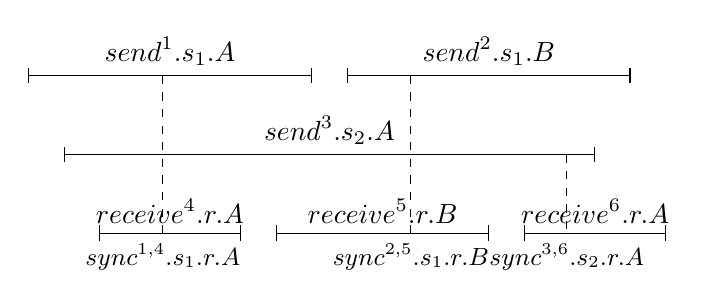
\begin{tikzpicture}[xscale = 0.9]
\draw[|-|] (0,0) -- node[above] {$\sm{send}^1.s_1\sm{.A}$} (4,0);
\draw[|-|] (4.5,0) -- node[above] {$\sm{send}^2.s_1\sm{.B}$} (8.5,0);
\draw[|-|] (0.5,-1) -- node[above] {$\sm{send}^3.s_2\sm{.A}$} (8,-1);
\draw[|-|] (1,-2) -- node[above] {$\sm{receive}^4.r.A$} (3,-2);
\draw[|-|] (3.5,-2) -- node[above] {$\sm{receive}^5.r.B$} (6.5,-2);
\draw[|-|] (7,-2) -- node[above] {$\sm{receive}^6.r.A$} (9,-2);
\draw (1.9,0) \X; \draw (1.9,-2) \X; 
\draw[dashed] (1.9,0) -- (1.9,-2); % sync 1 and 3
\draw (1.9,-2.3) node {\small $\sm{sync}^{1,4}.s_1.r.\sm{A}$};
\draw (5.4,0) \X; \draw (5.4,-2) \X; 
\draw[dashed] (5.4,0) -- (5.4,-2); % sync 4 and 5
\draw (5.4,-2.3) node {\small $\sm{sync}^{2,5}.s_1.r.\sm{B}$};
\draw (7.6,-1) \X; \draw (7.6,-2) \X; 
\draw (7.6,-2.3) node {\small $\sm{sync}^{3,6}.s_2.r.\sm{A}$};
\draw[dashed] (7.6,-1) -- (7.6,-2); % sync 2 and 6 
\end{tikzpicture}
\scalaMid
\end{center}
%% \caption{Timeline representing the synchronisation example.}
%% \label{fig:sync-timeline}
%% \end{figure}
%
Time goes from left to right in the diagram.  Each horizontal line represents
an operation execution, with the end points representing the \CSPM{begin} and
\CSPM{end} events.  A corresponding synchronisation history is written at the
bottom, where each pair of ``$\cross$''s, linked by a dashed vertical line,
illustrates a possible synchronisation point of the corresponding executions.

We considered only complete histories above.  We now generalise.  An
\emph{extension} of a (not necessarily complete) history~$h$ is formed by
adding zero or more |end| events corresponding to pending executions.  We
write $complete(h)$ for the subsequence of~$h$ formed by removing all |begin|
events of pending operation executions.
%
\begin{definition}
Let $h$ be a (not necessarily complete) history of the channel, and $h_s$ a
legal synchronisation history.  We say that $h_s$ is a \emph{synchronisation
  linearisation} of~$h$ if there is an extension~$h'$ of~$h$ such that $h_s$
is a synchronisation linearisation of $complete(h')$.  We say that $h$ is
synchronisation linearisable in this case.
%
We say that a synchronous channel is synchronisation linearisable if all of
its histories are synchronisation linearisable.
\end{definition}
%
Informally, the |end| events that are in~$h'$ but not in~$h$ correspond to
executions that have synchronised but not yet returned.

%% Thus a history (or trace) is synchronisation linearisable if it is possible
%% to identify synchronisation points with the desired properties.  This
%% corresponds to identifying which operation executions synchronise with one
%% another.

%% A more general definition is in~\cite{LL:synchronisation}.  In particular,
%% this includes the case where the synchronisation object maintains some state
%% between synchronisations, as we will require in
%% Section~\ref{sec:syncchan-closing}.

The definition is based on \emph{linearisation}~\cite{herlihy-wing}, the
standard correctness property for concurrent datatypes, where executions of
operations should appear to take place in a one-at-a-time order, each between
the beginning and end of that execution.  However, the two notions are
distinct: informally, synchronisation linearisation requires that operation
executions appear to take place in a two-at-a-time order.  More precisely,
synchronisation linearisation requires corresponding executions to overlap in
time.  A history where, say, a |send| returns before the corresponding
|receive| is invoked would not represent a correct synchronisation.  This
overlapping property cannot be captured directly with standard
linearisation~\cite{LL:synchronisation}.

%% The current model of the channel is (in the terminology
%% of~\cite{LL:synchronisation}) \emph{stateless}: no state is carried forward
%% from one synchronisation to another.  However, when we consider closing of the
%% channel, it will become \emph{stateful}, with two states, open or closed.
%% Other synchronisation objects have more interesting states.  \framebox{later?}

We now describe how we use model checking to test synchronisation
linearisability of the channel.  (We drop the execution identifiers from
events: they were just convenient in defining synchronisation linearisation.)
We create an instance |C| of the channel module from
Figure~\ref{fig:basic-CSP-model} .  Below, expressions of the form |C::v|
represent a value~|v| from this instance.
%
We create a processes that represent threads (with identities
from a set |ThreadID|): each thread repeatedly calls the send and receive
operations,
% (represented by events on CSP channels |C::beginSend| and |C::beginReceive|),
and waits for them to return:
% (on CSP channels |C::endSend| and |C::endReceive|).
%
\begin{cspm}
Thread(me) = 
  C::beginSend.me?x -> C::endSend.me?res -> Thread(me)
  [] C::beginReceive.me -> C::endReceive.me?res -> Thread(me)
Threads = **||| t : ThreadID @ Thread(t)
\end{cspm}
%
We build a process |System| that combines the threads with the channel (the
function |runWithAndHide| from the channel module runs its argument in
parallel with the module's internal processes, and hides the internal events):
\begin{cspm}
System = C::runWithAndHide(Threads)
\end{cspm}

We now build a CSP specification process that allows precisely the traces that
are synchronisation linearisable.  As above, we use events of the form
\CSPM{sync.t}$_1$\CSPM{.t}$_2$\CSPM{.x} to represent a synchronisation point
between sender~$\CSPMM{t}_1$ and receiver~$\CSPMM{t}_2$, passing data
value~|x|.  We build a \emph{lineariser} process for each thread as follows,
which ensures that the |sync| events occur between the corresponding |begin|
and |end| events (the approach is based on that for standard
linearisation~\cite{gavin:lock-free-queue}).
%
\begin{cspm}
Lin(t) = 
  C::beginSend.t?x -> sync.t?other!x -> C::endSend.t.SendSuccess -> Lin(t)
  [] C::beginReceive.t -> sync?other!t?x -> C::endReceive.t.ReceiveSuccess.x -> Lin(t)
\end{cspm}
%
When sending, the thread can synchronise with any other thread~|other|,
passing its value~|x|.  When receiving, the thread can synchronise with any
other thread, accepting that thread's value~|x|; this |x| is subsequently
returned by the operation execution.

We combine the |Lin| processes in parallel, with their natural
alphabets, so the linearisers for threads $\CSPMM{t}_1$ and $\CSPMM{t}_2$
synchronise on events of \CSPM{sync.t}$_1$\CSPM{.t}$_2$ and
\CSPM{sync.t}$_2$\CSPM{.t}$_1$.  
%
\begin{cspm}
alphaLin(t) =
  {|C::beginSend.t, C::endSend.t, C::beginReceive.t, C::endReceive.t|} £$\union$£
  {|sync.t.other, sync.other.t | other <- ThreadID-{t}|}
Spec£$_0$£ = **|| t <- ThreadID @ [alphaLin(t)] Lin(t)
\end{cspm} % £$\union$£
%
Thus each trace of |Spec|$_0$ represents an interleaving of a history of the
channel with a synchronisation history, as required by
Definition~\ref{def:sync-lin}.  By hiding the synchronisation points, we
obtain a process whose traces represent precisely those histories that are
synchronisation linearisable.  We can then use FDR to check that the system is
synchronisation linearisable.
%
\begin{cspm}
Spec = Spec£$_0$£ \ {|sync|}
assert Spec [T= System
\end{cspm}


%%%%%%%%%%%%%%%%%%%%%%%%%%%%%%%%%%%%%%%%%%%%%%%%%%%%%%%

We now consider our progress property, \emph{synchronisation
  progressibility}~\cite{LL:synchronisation}.  This property assumes that the
system scheduler is fair, in the sense that if a thread is continuously
runnable, it will eventually be scheduled.  However, the assumption allows for
unfortunate scheduling, or for a thread to be repeatedly preempted, for
example when competing with other threads to acquire a lock.  Most modern
schedulers are fair in this sense.
The following definition captures our fairness assumption.
%
\begin{definition}
Given an execution, we say that an operation execution is \emph{pending} if it
has been called but not yet returned.  We say that an operation execution is
\emph{blocked} in a particular state if it is unable to perform a step, for
example because it is trying to acquire a lock held by another thread, or
waiting to receive a signal from another thread.

We say that an infinite execution is \emph{fair} if each pending operation
execution either (a)~eventually returns, (b)~is blocked in infinitely many
states, or (c)~performs infinitely many steps.  We consider a system execution
that reaches a deadlocked state (where every pending operation is permanently
blocked) to be infinite (it is infinite in time), and hence fair (under~(b)).
\end{definition}

%%%%%

Synchronisation progressibility requires that, under this fairness assumption,
if a synchronisation is possible, some such synchronisation will happen, and
the threads become able to return.  If several alternative synchronisations
are possible, then synchronisation progressibility allows any to happen.
Informally, threads do not get stuck if there are synchronisations that could
occur.  For example, if three threads call, respectively, |send(4)|, |send(5)|
and |receive| on the channel, then synchronisation progressibility requires
that the receiver synchronises with one of the senders, and those two threads
return.

%%%%%

The following definition captures a maximal sequence of synchronisations that
might occur, given a particular history of the channel.
%
\begin{definition}
Given a history~$h$ of a channel, and a legal synchronisation history~$h_s$,
we say that $h_s$ is a \emph{maximal synchronisation linearisation} of~$h$ if:
(a)~$h_s$ is a synchronisation linearisation of~$h$; and (b)~no proper
extension $h_s \cat \seq{e}$ is a synchronisation linearisation of~$h$.
\end{definition}
%
For example, the history 
\begin{eqnarray*}
h & = &\seq{\beginSend^1.s_1.4,\, \beginSend^2.s_2.5,\, \beginReceive^3.r }
\end{eqnarray*}
has two maximal synchronisation linearisations
\[
h_s^1  =   \seq{\sync^{1,3}.s_1.r.4}, \qquad\mbox{and}\qquad
h_s^2  =  \seq{\sync^{2,3}.s_2.r.5},
\]
corresponding to the two possible synchronisations.  Each describes one
possibility for all the synchronisations that might happen. 

%%%%%

The following definition captures the $\End$ events that we would expect to
happen given a particular sequence of synchronisations.
%
\begin{definition}
Given a history~$h$ of the synchronisation object and a maximal
synchronisation linearisation~$h_s$, we say that an $\End$ event is
\emph{anticipated} if it does not appear in~$h$, but the corresponding $\sync$
event appears in~$h_s$.
\end{definition}
%
For the above histories~$h$ and~$h_s^1$, the events
$\endSend^1.s_1.\SendSuccess$ and $\endReceive^3.r.\ReceiveSuccess.4$  are
anticipated: assuming $h_s^1$ describes the synchronisations that happen, we
would expect those $\End$ events to occur; if they do not, that is a failure
of progress.

%%%%%

\begin{definition}
Let $h$ be a history of a channel.  We say that $h$ is \emph{synchronisation
  progressible} if, from the state reached after~$h$, for every fair infinite
execution with no new $\Begin$ events, there is a maximal synchronisation
  linearisation~$h_s$ of~$h$ such that every anticipated $\End$ event~$e$
  eventually happens.

We say that a channel is synchronisation progressible if all of its histories
are synchronisation progressible.
\end{definition}

For the earlier history~$h$, synchronisation progressibility requires that
either $\endSend^1.s_1.\SendSuccess$ and $\endReceive^3.r.\ReceiveSuccess.4$
eventually happen (corresponding to~$h_s^1$), or $\endSend^2.s_2.\SendSuccess$
and $\endReceive^3.r.\ReceiveSuccess.5$ eventually happen (corresponding
to~$h_s^2$): one of the synchronisations should happen, and then the relevant
operations should return.

On the other hand, for the history $\trace{\beginSend^1.s.4}$, the only
maximal synchronisation linearisation is $\trace{}$, for which there are no
anticipated returns, and so synchronisation progressibility is vacuously
satisfied: it is fine for the |send| to get stuck in this case, since there is
no |receive| with which it could synchronise.

%%%%%%%%%%%%%%%%%%%%%%%%%%%%%%%%%%%%%%%%%%%%%%%%%%%%%%%

%% We now consider how to test for synchronisation progressibility using CSP and
%% FDR.  We need to check that anticipated $\End$ events are available, i.e.~not
%% refused.  To do this, we require that the system model is divergence-free,
%% since FDR models do not accurately capture refusal information in divergent
%% states.  However, as we will see, this is the case.   

We can test our CSP model for synchronisation progressibility by repeating the
earlier refinement test, except in the failures-divergences model (which
implies the refinement in the traces model):
%
\begin{cspm}
assert Spec [FD= System
\end{cspm}
%
Note that this test requires that the system cannot diverge, and so must
eventually reach a stable state.  The failures-divergences model records
refusal information only in stable states.  This reflects our assumption about
scheduling: unstable states are transient, because there must be some internal
step by a thread that is possible and that will be scheduled.  If a
synchronisation is possible, then the specification will reach a state where
relevant |end| events are available (i.e.~not refused).  The test, then,
requires that in stable states, the system also makes those |end| events
available.  If, in fact, there are two or more possible synchronisations, the
specification will choose nondeterministically which to perform, and so the
system may likewise perform any such synchronisations.

The property of \emph{lock freedom}~\cite{Herlihy-Shavit} requires that
eventually some thread returns, assuming the scheduler repeatedly schedules
threads.  Synchronisation progressibility is not the same as lock freedom,
because lock freedom does not assume that the scheduler is fair.  Indeed, SCL
channels are not lock-free, because of the use of a lock: if one thread
obtains the lock, and then the scheduler only schedules other threads, those
other threads would be blocked trying to obtain the lock, and so no thread
would return.  However, under our assumption of fair scheduling, the thread
holding the lock would eventually be scheduled and so release the lock.

The property of \emph{wait freedom} requires that if a particular thread is
repeatedly scheduled, it eventually returns.  The property of
\emph{obstruction freedom} requires that if a thread executes in isolation
(i.e.~no other thread is scheduled), then it eventually returns.  SCL channels
are neither wait-free not obstruction-free, for the same reason as above.
Hence synchronisation progressibility is also distinct from these two
properties.

%%%%%%%%%%%%%%%%%%%%%%%%%%%%%%%%%%%%%%%%%%%%%%%%%%%%%%%

%% We can also test the same refinement in the stable failures model (which
%% implies the refinement in the traces model).
%% %
%% \begin{cspm}
%% assert Spec [F= System
%% \end{cspm}
%% %
%% This captures a useful progress property, which says that if a synchronisation
%% is possible (i.e.~there is at least one |send| and one |receive| operation
%% that have been called but not yet returned), then some such synchronisation
%% must happen (since an internal |sync| event is available), and so the relevant
%% threads reach a state where they can return.  (If several different
%% synchronisations are possible, then the refinement test allows any to happen.)
%% Informally, threads don't get stuck unnecessarily.  We call this property
%% \emph{synchronisation progressiblity}~\cite{LL:synchronisation}.  This
%% property corresponds to an assumption that the scheduler is fair in the sense
%% that if a thread is continuously runnable, it will eventually be scheduled and
%% so able to make progress; however, this doesn't prevent the thread being
%% repeatedly preempted, for example when competing with other threads to acquire
%% a lock. 

Finally, note that the fact that |System| does not diverge verifies that no
thread in the implementation throws an exception. 

%% Finally, as discussed above, we can test that |System| does not diverge, to
%% verify that no thread in the implementation throws an exception.  Further,
%% this verifies that threads cannot perform an infinite amount of internal
%% activity without any thread returning.  This test can be combined with the
%% previous by testing for refinement in the failures-divergences model.
%% %
%% \begin{cspm}
%% assert Spec [FD= System
%% \end{cspm}

It turns out that our specification is equivalent to that of Welch and
Martin~\cite{welch-martin} when restricted to non-shared channels (which they
consider).  However, we consider our specification to be an instance of a more
general pattern, for synchronisation objects, rather than a single-purpose
specification.
 % Analysing basic channel
\subsection{Closing channels}
\label{sec:syncchan-closing}

\inlineScala

We now consider the closing of SCL channels.  Recall that, after the channel
has been closed, a |send| or |receive| execution fails and throws a |Closed|
exception.

Implementing the |close| operation correctly proved harder than expected.  An
earlier version of the implementation suffered from a bug involving three
threads acting concurrently: thread~$A$ calls |send(x)|, thread~$B$ calls
|receive|, and thread~$C$ calls |close|.  Under certain conditions, it was
possible for thread~$B$ to return successfully, having received~|x|, but for
thread~$A$ to see the channel closed, and so throw a |Closed| exception.  We
consider this behaviour to be incorrect: either both~$A$ and~$B$ should think
the communication has succeeded, or both should throw |Closed| exceptions.

%%%%%%%%%% Implementation

The SCL implementation uses a boolean variable |isChanClosed| that records
whether the channel is closed.  The |close| operation sets this variable, and
signals to all the threads waiting on conditions.
\begin{scala}
def close = lock.mutex{
  if(!isChanClosed){isChanClosed = true; slotEmptied.signalAll(); slotFull.signalAll(); continue.signalAll()}
}
\end{scala}

The implementation also uses a variable |receiversWaiting|, which records how
many receivers are currently waiting to receive a value. 

Figure~\ref{fig:close-send-receive} gives code to show how |send| and
|receive| deal with the channel being closed.  (Note: this is still a large
simplification of the full code, which supports alts and the timed
operations.)

%%%%%

\begin{figure}
\begin{minipage}[t]{80mm}
\begin{scala}
def send(x: A) = lock.mutex{
  while(status != Empty && !isChanClosed)
    slotEmptied.await()  
  if(isChanClosed) throw new Closed
  value = x; status = Filled
  if(receiversWaiting > 0) slotFull.signal()
  continue.await()  
  if(status == Read){ 
    status = Empty; slotEmptied.signal() }
  else{ 
    assert(isChanClosed)
    if(receiversWaiting == 0) throw new Closed }
}
\end{scala}
\end{minipage}
%
\begin{minipage}[t]{75mm}
\begin{scala}
def receive(): A = lock.mutex{
  if(isChanClosed) throw new Closed
  while(status != Filled){
    receiversWaiting += 1; slotFull.await()
    receiversWaiting -= 1
    if(status != Filled && isChanClosed)
      throw new Closed
  }
  status = Read; continue.signal(); value
}
\end{scala}
\end{minipage}
\caption{Code for deadling with closed channels when sending and receiving.}
\label{fig:close-send-receive}
\end{figure}

%%%%%

When a thread calls |send| or |receive|, if |isChanClosed| is set, it throws a
|Closed| exception.  Likewise, if a sending thread waits on |slotEmptied|, it
performs a similar check when it receives a signal.  

If a receiving thread waits on |slotFull|, when it receives a signal, it first
checks whether |status| holds |Filled|.  If so, it continues as described
earlier: thus we prioritise completing the communication over checking whether
the channel has been closed (this seems necessary for correct interaction with
alts).
%
%% More precisely, an alt might have filled the slot, which implies it has
%% performed the computation to calculate the value: at this point, it is
%% committed to the communication. 
If |status| does not hold |Filled|, the thread checks whether the channel has
been closed, and if so throws an exception; otherwise, it waits again on
|slotFull|.

If a sending thread waits on |continue|, when it receives a signal, it first
checks whether |status| holds |Read|, and if so continues as described
earlier.  Otherwise, it must be the case that |isChanClosed| has been set (the
SCL implementation asserts this, and the CSP analysis below checks this).
However, if there is a receiver waiting (as recorded by |receiversWaiting|),
then that receiver will eventually return the value being sent, so the sending
thread should also return successfully.  If there is no waiting receiver, the
sending thread throws a |Closed| exception.
%
%% \begin{scala}
%%   continue.await()  
%%   if(status == Read){ status = Empty; slotEmptied.signal() }
%%   else{ assert(isChanClosed); if(receiversWaiting == 0) throw new Closed }
%% \end{scala}

The precise order of checks in the previous paragraphs is rather subtle.  This
is where the earlier implementation went wrong.  Previously, when the waiting
thread received a signal, it \emph{first} checked |isChanClosed|, and if it
was set, threw a |Closed| exception.  This could be wrong for a couple of
reasons, as illustrated in Figure~\ref{fig:old-impl-error}.
%
\begin{itemize}
\item
In the top part of the figure, a receiving thread reads and returns the
sending thread's value, indicating that it has correctly synchronised.  Then
the channel is closed.  If the |send| first checks |isChanClosed|, it will
throw a |Closed| exception.  This is an error: either both threads should
succeed, or both should see the channel had closed, and fail.  The correct
version (Figure~\ref{fig:close-send-receive}) instead reads |status| first,
and returns correctly.

\item
The bottom part of the figure is similar, but the channel is closed and the
|send| continues \emph{before} the |receive| reads the sender's value.  If the
|send| first checks |isChanClosed| (and maybe |status|), it will throw a
|Closed| exception, even though the |receive| will subsequently return the
sender's value.  This is again an error.  The correct version instead finds
$\sm{receiversWaiting} > 0$, and so returns correctly.
\end{itemize}
This correct version was found with the help of the model checking described
below.


%%%%%%%%%%

\begin{figure}
\def\height{10.5}
\def\width{6}
%%%%%
\begin{tikzpicture}[yscale = 0.5, xscale = 0.9, >= angle 60]
\draw (0,0) node[draw](send){\scalashape send};
\draw (send) -- ++ (0,-\height);
\draw (\width,0) node[draw](receive){\scalashape receive};
\draw (receive) -- ++ (0,-\height);
\draw (12,0) node[draw](close){\scalashape close};
\draw (close) -- ++ (0,-\height);
%
%\draw (receive) ++(0,-1) node[right]{\ldots; \scalashape slotFull.await()};
%
\draw (send)++(0,-1) node[right]{\ldots};
\draw (send)++(0,-2) node[right]{
  set {\scalashape value = x}, {\scalashape status = Filled}};
%\draw[->] (0,-3.7) -- node[above]{\scalashape slotFull.signal()}  (\width,-3.7);
\draw (send)++(0,-3) node[right]{\ldots; \scalashape continue.await()};
%
\draw (receive) ++ (0,-4) node[right]{
  \ldots; read {\scalashape status = Filled}};
\draw (receive) ++ (0,-5) node[right]{set {\scalashape status = Read};
  \ldots};
\draw (receive) ++ (0,-6) node[right]{ \scalashape continue.signal()};
\draw[->] (receive)++(0,-6) --  (0,-6);
\draw (receive) ++ (0,-7) node[right]{return {\scalashape value}};
%
\draw (close)++(0,-8) node[right]{set {\scalashape isChanClosed = true}; \ldots};
%
\draw (send) ++ (0,-9) node[right]{read {\scalashape isChanClosed = true}};
\draw (send) ++ (0,-10) node[right]{throw {\scalashape Closed} exception};
\end{tikzpicture}

\bigskip

%%%%%

\def\height{11.5}
\begin{tikzpicture}[yscale = 0.5, xscale = 0.9, >= angle 60]
\draw (0,0) node[draw](send){\scalashape send};
\draw (send) -- ++ (0,-\height);
\draw (\width,0) node[draw](receive){\scalashape receive};
\draw (receive) -- ++ (0,-\height);
\draw (12,0) node[draw](close){\scalashape close};
\draw (close) -- ++ (0,-\height);
%
\draw (receive) ++(0,-1) node[right]{\ldots; \scalashape slotFull.await()};
%
\draw (send)++(0,-2) node[right]{\ldots};
\draw (send)++(0,-3) node[right]{
  set {\scalashape value = x}, {\scalashape status = Filled}};
\draw (send)++(0,-4) node[right] (sig1) {\scalashape slotFull.signal()};
\draw[->] (sig1) --  (\width,-4);
\draw (send)++(0,-5) node[right]{\ldots; \scalashape continue.await()};
%
\draw (close)++(0,-6) node[right]{set {\scalashape isChanClosed = true};
  \ldots};
%% \draw(close)++(0,-7) node[right]{\scalashape slotFull.signalAll()};
%% \draw[->] (close)++(0,-7) -- (\width,-7);
\draw(close)++(0,-7) node[right]{\scalashape continue.signalAll()};
\draw[->] (close)++(0,-7) -- (0,-7);
%
\draw (send) ++ (0,-8) node[right]{read {\scalashape isChanClosed = true}};
\draw (send) ++ (0,-9) node[right]{throw {\scalashape Closed} exception};
%
\draw (receive) ++ (0,-10) node[right]{
  \ldots; read {\scalashape status = Filled}; \ldots};
\draw (receive) ++ (0,-11) node[right]{return {\scalashape value}};
%

\end{tikzpicture}

\caption{Illustration of errors that arise in the earlier implementation.
  Several steps are elided, for brevity.}
\label{fig:old-impl-error}
\end{figure}

%%%%%%%%%% Model

\inlineCSP

Adapting the CSP model to model closing of channels is straightforward.  The
|endSend| and |endReceive| channels are extended to allow a result |Closed|,
corresponding to the \SCALA{Closed} exception.  The \SCALA{close} operation is
modelled as for earlier operations, framed by events on channels |beginClose|
and |endClosed|.

%%%%%%%%%% Testing

To analyse this extended model, we adapt the |System| process from earlier to
also allow threads to close channels.  

The channel specification in Section~\ref{sec:syncchan-analysis-1} is (in the
terminology of~\cite{LL:synchronisation}) \emph{stateless}: no state is
carried forward from one synchronisation to another.  However, when we
consider closing of the channel, it becomes \emph{stateful}, with two states,
open or closed.  (Other synchronisation objects have more interesting states.)
The definition of synchronisation linearisation requires the synchronisation
history to be consistent with the state. 

Our specification will treat \SCALA{close} as a linearisable operation: it
will appear to take place atomically, at some point, called the
\emph{linearisation point}, between the |beginClose| and |endClose| events.
(Equivalently, the |close| operation can be thought of as a unary
synchronisation, involving a single thread, in contrast to the earlier binary
synchronisations.)  We require that the history is consistent with this
closing: synchronisations between sends and receives should take place before
the linearisation point of the close; and sends and receives that return
|Closed| should be linearised after the close.

We use a CSP event |close.t| to represent the linearisation point of a
\SCALA{close} operation by thread~|t|.  Further, we use an event |closed.t| to
represent the linearisation point of a send or receive operation by thread~|t|
that returns |Closed| because it finds that the channel is closed.

Within the specification, the state of the channel is recorded by the process
|ChanSpec|.  When the channel is open, it allows threads to synchronise, or
allows a thread to close the channel.  When the channel is closed, it allows
linearisation points of sends or receives that return |Closed|, or allows the
linearisation point of another |close| operation (a |close| operation on a
channel that is already closed has no effect).
%
\begin{cspm}
ChanSpec = sync?t1?t2?x -> ChanSpec [] close?t -> ChanSpecClosed
ChanSpecClosed = isClosed?t -> ChanSpecClosed [] close?t -> ChanSpecClosed
alphaChanSpec = {|sync, close, isClosed|} 
\end{cspm}

We adapt the lineariser processes to reflect the closing of channels.  A
sending thread can either synchronise with another thread, as before, or find
that the channel is closed and so return the |Closed| value.  (The
|SendingLin| process that describes this is parameterised by the corresponding
|endSend| channel, to facilitate extension to the timed operations later.)
Receiving is treated similarly.  Further, the linearisation point for a
\SCALA{close} operation can take place between |beginClose| and |endClose|
events.
%
%\pagebreak[1]
%\begin{mysamepage}
\begin{cspm}
Lin(t) = 
  C::beginSend.t?x -> SendingLin(t, x, C::endSend.t)
  [] C::beginReceive.t -> ReceivingLin(t, C::endReceive.t)
  [] C::beginClose.t -> close.t -> C::endClose.t -> Lin(t)

SendingLin(t, x, endChan) = 
  sync.t?other!x -> endChan.SendSuccess -> Lin(t)
  [] isClosed.t -> endChan.Closed -> Lin(t)

ReceivingLin(t, endChan) =  
  sync?other!t?x -> endChan.ReceiveSuccess.x -> Lin(t)
  [] isClosed.t -> endChan.Closed -> Lin(t)
\end{cspm}
%\end{mysamepage}


\begin{figure}
\begin{center}
\def\height{10mm} % height of boxes
\begin{tikzpicture}[yscale = 1.5]
\draw (0,0) node[draw, minimum height = \height](lin1){\cspmstyle Lin(T1)};
\draw (0,-2) node[draw, minimum height = \height](lin2){\cspmstyle Lin(T2)};
\draw (5.5,-1) node[draw, minimum height = \height](chanSpec){
  \cspmstyle ChanSpec};
% inter-process events
\draw (lin1) -- (lin2); 
\fill (0,-1)  circle(1.5pt) coordinate (T1);
\draw (T1) -- node[above]{{\cspmstyle sync.T1.T2}, {\cspmstyle sync.T2.T1}}
   (chanSpec);
\draw (lin1) -| node[near start, above]{
  {\cspmstyle close.T1}, {\cspmstyle isClosed.T1}}  (chanSpec);
\draw (lin2) -| node[near start, below]{
  {\cspmstyle close.T2}, {\cspmstyle isClosed.T2}}  (chanSpec);
% outer box
\draw (-1,0.5) -- (6.7,0.5) -- (6.7,-2.5) -- (-1,-2.5) -- (-1,0.5);
% begin, end events
\draw (-3.2,0) node (be1) {
  \begin{tabular}{r@{}}
  \CSPM{(begin}\m\CSPM{end)Send}.\CSPM{T1} \\ 
  \CSPM{(begin}\m\CSPM{end)Receive}.\CSPM{T1} \\
  \CSPM{(begin}\m\CSPM{end)Close}.\CSPM{T1}
  \end{tabular}};
\draw(be1.east) -- (lin1);
\draw (-3.2,-2) node (be2) {
  \begin{tabular}{r@{}}
  \CSPM{(begin}\m\CSPM{end)Send}.\CSPM{T2} \\ 
  \CSPM{(begin}\m\CSPM{end)Receive}.\CSPM{T2} \\
  \CSPM{(begin}\m\CSPM{end)Close}.\CSPM{T2}
  \end{tabular}};
\draw(be2.east) -- (lin2);
\end{tikzpicture}
\end{center}
\caption{Construction of the specification process, with two threads.  We use
  BNF-style notation to capture channels with similar names; for example, we
  write ``{\cspmstyle (begin}\m{\cspmstyle end)Send}'' to denote the
  {\cspmstyle beginSend} and {\cspmstyle endSend} channels.}
\label{fig:closable-spec}
\end{figure}

We combine the linearisers as before (with suitably extended alphabets).  We
then synchronise them with |ChanSpec| on the relevant events.
events.
%
\begin{cspm}
AllLins = **|| t <- ThreadID @ [alphaLin(t)] Lin(t)
Spec£$_0$£ = AllLins [| alphaChanSpec |] ChanSpec
\end{cspm}
%
This is illustrated in Figure~\ref{fig:closable-spec} in the case of two
threads.

%
For example, |Spec|$_0$ allows traces such as
\[
\begin{align}
\trace{
  \CSPMM{C::beginSend.T1.A},\; \CSPMM{C::beginReceive.T2},\;
  \CSPMM{C::beginClose.T3},\; 
  \CSPMM{sync.T1.T2.A},\; \CSPMM{close.T3},
\\
\qquad  \CSPMM{C::endSend.T1.SendSuccess},\; 
  \CSPMM{C::endReceive.T2.ReceiveSuccess.A},\; \CSPMM{C::endClose.T3}
}.
\end{align}
\]
Here |T1| is trying to send, |T2| is trying to receive, and |T3| is trying to
close the channel; the synchronisation between~|T1| and~|T2| happens before
the |close| has an effect, so the threads successfully communicate.  But
|Spec|$_0$ also allows traces such as

\[
\begin{align}
\trace{
  \CSPMM{C::beginSend.T1.A},\; \CSPMM{C::beginReceive.T2},\;
  \CSPMM{C::beginClose.T3},\; 
  \CSPMM{close.T3},\; \CSPMM{isClosed.T1},\; \CSPMM{isClosed.T2},
\\
\qquad  \CSPMM{C::endSend.T1.Closed},\; 
  \CSPMM{C::endReceive.T2.Closed},\; \CSPMM{C::endClose.T3}
}.
\end{align}
\]
Here the channel is closed before |T1| and~|T2| can synchronise, so both
return the |Closed| value.

We can then define the specification process
\begin{cspm}
Spec = Spec£$_0$£ \ alphaChanSpec
\end{cspm}
Thus |Spec| allows all traces, containing the |begin| and |end| events, that
are synchronisation linearisable.  So testing \CSPM{Spec [T= System}
%] bracket match hack
verifies synchronisation linearisability for this system.  Performing the
corresponding test in the stable failures model also verifies synchronisation
progressibility.  Finally, performing the test in the failures-divergences
model also verifies that all assertions in the code pass, and that threads
cannot perform an infinite amount of internal activity without a thread
returning.

%%%%%%%%%%%%%%%%%%%%%%%%%%%%%%%%%%%%%%%%%%%%%%%%%%%%%%%

\subsection{Timed operations}
\label{sec:syncchan-timed}

\inlineScala

We now consider the timed send and receive operations on channels.  

The SCL conditions described earlier provide a timed wait operation: the
thread waits until either it receives a signal, or the time is elapsed; the
operation returns a boolean indicating whether a signal was received.  The
timed send and receive operations are based around this. 

The |sendWithin(duration)(x)| operation initially waits on |slotEmptied| until
either |status| holds |Empty| or the channel is closed (which it rechecks when
it receives a signal), or the deadline is reached.  If the channel is closed,
it throws a |Closed| exception.  If it timed out, it returns |false|.
Otherwise, it continues as in the untimed operation, except it waits on
|continue| until at most |duration| after the initial call.  If it then finds
that |status| is |Read|, then the send has been successful; it continues as in
the untimed operation, and returns |true|.  Otherwise |status| must still hold
|Filled| and |value| must still hold~|x| (the implementation asserts this, and
the analysis below checks this).  If the channel is closed, it continues as in
the untimed operation.  Otherwise, it must have timed out, so it sets |status|
to |Empty| to clear its value, signals to any thread waiting on |slotEmptied|,
and returns |false|.

The |receiveWithin(duration)| operation acts much as the untimed version,
except it waits on |slotFull| until at most |duration| after the initial
call.  If it then finds that |status| holds |Filled|, it continues as in the
untimed case, returning a suitable |Some| value.  If the channel is closed, it
throws a |Closed| exception.  Otherwise it must have timed out, so returns
|None|.  

%%%%% Modelling

We now describe the CSP model of these operations.  Our model and subsequent
analysis do not consider absolute time; thus we abstract away from the
duration of a timed send or receive.  The difficult part of the implementation
is getting the synchronisations right, rather than the length of the delay.

The CSP model of an SCL monitor, described in
Section~\ref{sec:basic-csp-model}, also models timed waits, via a function
|TimedAwait|.  A thread that calls this function might receive a signal, as
for untimed waits.  In addition, it can time out.  Thus we model that such
threads can eventually time out, but, as noted above, don't model the length
of the delay.


%% earlier, can be extended to also
%% model timed waits.  It records which threads are doing timed waits on which
%% conditions.  Such threads can receive a signal, as for untimed waits.  In
%% addition, they can time out, and subsequently acquire the lock on the monitor.
%% Thus we model that such threads can eventually time out, but, as noted above,
%% don't model the length of the delay.
%% , so we abstract away from the duration of a timed send or
%% receive.  The difficult part of the implementation is getting the
%% synchronisations right, rather than the length of the delay.

The |sendWithin| and |receiveWithin| operations can then be modelled in CSP
much as before, using these timed waits.


%%%%% Analysis

\inlineCSP

We adapt the specification of synchronisation linearisability as follows.  We
introduce events |timeout.t| to represent the linearisation point of a
\SCALA{sendWithin} or \SCALA{receiveWithin} operation by thread~|t| that times
out (again abstracting away from the length of the delay).  We then adapt the
definition of the lineariser processes for these operations as follows, adding
the possibility of such a time out to the possibilities of the untimed
operations.
%
\begin{cspm}
Lin(t) = 
  ... -- as before
  [] C::beginSendWithin.t?x -> SendingWithinLin(t, x, C::endSendWithin.t)
  [] C::beginReceiveWithin.t -> ReceivingWithinLin(t, C::endReceiveWithin.t)

SendingWithinLin(t, x, endChan) = 
  SendingLin(t, x, endChan)
  [] timeout.t -> endChan.Timeout -> Lin(t)

ReceivingWithinLin(t, endChan) = 
  ReceivingLin(t, endChan) 
  [] timeout.t -> endChan.Timeout -> Lin(t)
\end{cspm}
%
Further, we adapt the |ChanSpec| process to allow |timeout| events only before
the channel is closed.  The rest of the construction and checks are then as
before. 

\begin{window}[2,r,{
%
\vspace{0.5ex}
\begin{tabular}[b]{\|cccc\|}
Model & Threads & States  & Time\\
FD & 3  & 1.23M & 3.6s\\
FD & 4 & 92.5M  & 43s \\
F & 5 & 7.22B & 34min 
\end{tabular}
%\vspace{1ex}
},]
%
The table to the right gives statistics about the number of states explored
and the times taken to perform these checks, in different models, and for
different numbers of threads.  Each test used two data values (and this is the
case for all later checks reported in this paper).  All
experiments in this paper were performed on a 32-core server (two 2.1GHz
Intel(R) Xeon(R) Gold 6130 CPUs with hyperthreading enabled, with 512GB of
RAM).  The check with 5 threads in the failures-divergences model was beyond
the limits of this machine.  As is normally the case, the state space, and
hence the checking time, grows rapidly with the number of threads.   
\end{window}

%% It is worth mentioning an alternative approach, which turns out not to work
%% in this case.  For standard concurrent datatypes, linearisability is often
%% verified by identifying \emph{linearisation points}: specific points in the
%% program code where an operation execution appears to take place.  By
%% analogy, can we identify \emph{synchronisation points} in the program code
%% for each operation, where the thread is aware of the result of the
%% execution, and then capture the correctness condition in terms of these
%% synchronisation points?  More precisely, we would like identify particular
%% events in the thread processes that represent the linearisation points.

%% This idea won't work in this case, essentially because the synchronisation
%% point for one thread might depend upon what happens in other threads, whereas
%% this idea requires \emph{fixed} synchronisation points.  The synchronisation
%% point for the sending thread would have to be after it receives the signal on
%% \SCALA{continue} and regains the lock, because it doesn't know the result of
%% the synchronisation before this; but this might be too late, because the
%% channel might have been closed before it obtained the lock, and so the
%% synchronisation would appear incorrect.
 % Closing channels
\section{Alts}
\label{sec:alt}

\inlineScala

We now consider alts.  We start by describing the high-level interactions
between an alt and channels, and how those interactions are implemented within
alts and channels.  We then outline how these interactions are modelled in
CSP, and describe a direct analysis of an alt and associated channels.

%%%%%%%%%%%%%%%%%%%%%%%%%%%%%%%%%%%%%%%%%%%%%%%%%%%%%%%

\subsection{High-level design}

We describe the interactions between an alt and relevant channels via operation
calls.  We call this the \emph{alt protocol}. 

When an alt runs, it starts by registering, in turn, with each of the relevant
ports whose guard evaluates to |true|.  This asks the port whether it is ready
to communicate.  The alt calls an operation
%
\begin{scala}
def registerIn(alt: AltT, index: Int, iter: Int): RegisterInResult[A]  
\end{scala}
%
on each of its inports, where |alt| is a reference to the calling alt, |index|
is the index of the branch within the alt, and |iter| is an iteration number
within a |serve| construct (used only for assertions).  The operation returns a
result of type |RegisterInResult[A]|, where |A| is the type of data passed by
the port, of one of the following forms.
%
\begin{description}
\item[\rm{\scalastyle RegisterInSuccess(x)}:] the port is willing to
  communicate, and the alt has received~|x| from it;

\item[\rm{\scalastyle RegisterInWaiting}:] the port is not currently willing to
  communicate (but the registration has been recorded); 

\item[\rm{\scalastyle RegisterInClosed}:] the port has been closed.
\end{description}
%
Similarly, the alt calls an operation
%
\begin{scala}
def registerOut(alt: AltT, index: Int, iter: Int, value: () => A): RegisterOutResult
\end{scala}
on each of its outports, where |alt|, |index| and |iter| are as for
|registerIn|, and |value| is a computation that, when evaluated, produces the
value to be sent.  The operation returns a result of one of the following
forms.
%
\begin{description}
\item[\rm{\scalastyle RegisterOutSuccess}:] the port is willing to
  communicate, and the alt has sent it a value;

\item[\rm{\scalastyle RegisterOutWaiting}:] the port is not currently willing to
  communicate (but the registration has been recorded); 

\item[\rm{\scalastyle RegisterOutClosed}:] the port has been closed.
\end{description}

If one of the registrations is successful, the alt deregisters from the
waiting branches, via operations |deregisterIn| and |deregisterOut|.  It then
executes the continuation of the successful branch.  

\def\IP{\emph{IP}}
\def\OP{\emph{OP}}

Figure~\ref{fig:alt-1} gives an example: an alt first registers unsuccessfully
with an inport~\IP; then it registers successfully with an outport~\OP; and
finally it deregisters from~\IP.

%%%%%

\begin{figure}
\begin{center}
%\unScalaMid
\def\height{5.5} % height of sequence diagram
\def\gap{3.5} % gap between columns
\begin{tikzpicture}[yscale = 0.8, >= angle 60]
\draw (0,0) node[draw](alt){Alt};
\draw (alt) -- ++ (0,-\height);
\draw (alt)++(\gap,0) node[draw](c1){\IP};
\draw (c1) -- ++(0,-\height);
\draw (c1)++(\gap,0) node[draw](c2){\OP};
\draw (c2) -- ++(0,-\height);
% Register with IP
\draw[->] (alt)++(0,-1) -- node[above]{\scalashape\small registerIn}
  ++ (\gap,0);
\draw[<-] (alt)++(0,-2) -- node[above]{\scalashape\small RegisterInWaiting} 
  ++ (\gap,0);
% Register with OP
\draw[->] (alt)++(0,-3) -- node[above, near end]{\scalashape\small registerOut}
  ++ (2*\gap,0);
\draw[<-] (alt)++(0,-4) -- 
  node[above, near end]{\scalashape\small RegisterOutSuccess}
  ++ (2*\gap,0);
% Deregister with IP
\draw[->] (alt)++(0,-5) -- node[above]{\scalashape\small deregisterIn}
  ++ (\gap,0);
\end{tikzpicture}
\end{center}
\caption{Sequence diagram illustrating an alt that registers successfully with
  a port. \label{fig:alt-1}}
\end{figure}

%%%%%

If no registration is successful, and the alt finds that every port is closed
or has a guard that is false, then it throws an |AltAbort| exception.
Otherwise, it waits for a callback from one of the ports with which it is
registered, of one of the following forms.
%
\begin{itemize}
\item If the alt is registered at the inport of a channel, and another thread
  tries to send on the channel, it calls
\begin{scala}
def maybeReceive(value: A, index: Int, iter: Int): Boolean
\end{scala}
%
on the alt, where |value| is the value it is trying to send to the alt, and
|index| and |iter| match the values provided during registration.  This asks
the alt whether it is still willing to receive from the inport.

\item If the alt is registered at the outport of a channel, and another thread
  tries to receive on the channel, it calls
%
\begin{scala}
def maybeSend[A](index: Int, iter: Int): Option[A]
\end{scala}
%
This asks the alt whether it is still willing to send a value to the inport.

\item If another thread closes the channel, it calls 
%
\begin{scala}
def portClosed(index: Int, iter: Int)
\end{scala}
\end{itemize}

If the alt receives a call of |maybeReceive| or |maybeSend|, it responds
positively to the first such call, returning |true| to a |maybeReceive|, or
|Some(x)| to a |maybeSend|, where~|x| is the value it sends.  It then
deregisters from the remaining branches.  
%
Finally, the alt
executes the continuation of the successful branch.
%
Figure~\ref{fig:alt-2} gives an example of a successful callback of
|maybeSend| from an outport with which the alt is registered.

\begin{figure}
\begin{center}
%\unScalaMid
\def\height{7.5} % height of sequence diagram
\def\gap{3.5} % gap between columns
\begin{tikzpicture}[yscale = 0.8, >= angle 60]
\draw (0,0) node[draw](alt){Alt};
\draw (alt) -- ++ (0,-\height);
\draw (alt)++(\gap,0) node[draw](c1){\IP};
\draw (c1) -- ++(0,-\height);
\draw (c1)++(\gap,0) node[draw](c2){\OP};
\draw (c2) -- ++(0,-\height);
% Register with IP
\draw[->] (alt)++(0,-1) -- node[above]{\scalashape\small registerIn}
  ++ (\gap,0);
\draw[<-] (alt)++(0,-2) -- node[above]{\scalashape\small RegisterInWaiting} 
  ++ (\gap,0);
% Register with OP
\draw[->] (alt)++(0,-3) -- node[above, near end]{\scalashape\small registerOut}
  ++ (2*\gap,0);
\draw[<-] (alt)++(0,-4) -- 
  node[above, near end]{\scalashape\small RegisterOutWaiting}
  ++ (2*\gap,0);
% Call back
\draw[<-] (alt)++(0,-5) -- node[above, near end]{\scalashape\small maybeSend}
  ++ (2*\gap,0);
\draw[->] (alt)++(0,-6) -- node[above, near end]{\scalashape\small Some(x)}
  ++ (2*\gap,0);
% Deregister with IP
\draw[->] (alt)++(0,-7) -- node[above]{\scalashape\small deregisterIn}
  ++ (\gap,0);
\end{tikzpicture}
\end{center}
\caption{Sequence diagram illustrating a successful callback from a
  port.  \label{fig:alt-2}}
\end{figure}

%%%%%

If the alt receives multiple callbacks to |maybeReceive| or |maybeSend|
(including during deregistration), it responds negatively to all except the
first, returning |false| or |None|, respectively.
%
If all the channels with which the alt is registered call |portClosed|, the
alt throws an |AltAbort|. 

%%%%%%%%%%%%%%%%%%%%%%%%%%%%%%%%%%%%%%%%%%%%%%%%%%%%%%%%%%%%

\subsection{Implementation details}

We now describe some details of the implementation.  Below we will use the
term ``alt-thread'' for the thread that is running the alt, and
``channel-thread'' for a thread performing an operation in a channel that
makes a callback to the alt. 

Each call of an operation on a channel (registering or deregistering) uses that
channel's lock, to avoid races.  

The implementation of the alt is based on a monitor, more specifically a
monitor provided by the Java Virtual Machine (JVM).  (JVM monitors are more
efficient than SCL monitors, because they are implemented directly in the JVM;
however, they do not allow targeting of signals.)  

The alt-thread holds the alt's lock throughout the registration phase.  Each
callback operation has to obtain this lock, so those operations are blocked
until registration is complete. 

However, it would be a mistake for the alt-thread to continue to hold the
alt's lock during deregistration, for this could lead to deadlocks.  Suppose
it did continue to hold the lock, and consider the case that the alt-thread is
trying to deregister from channel~$c$, at the same time that a channel-thread
is trying to perform a callback from~$c$: the channel-thread holds the lock
on~$c$, so the deregistration would be blocked; but the alt-thread holds the
lock on the alt, so the callback would be blocked.  The alt-thread therefore
releases the lock during deregistration. 

The implementation uses a variable |done| that is set to |true| when a
branch is found that is willing to communicate, either during registration or
as the result of a callback.  If a callback of |maybeSend| or |maybeReceive|
finds that |done| is |true|, it can return a negative result.  Otherwise, it
stores relevant information (like the value it is sending in the case of
|maybeReceive|, and the index of the relevant branch), evaluates the value to
be received in the case of |maybeSend|, sets |done| to |true|, signals to the
waiting alt-thread, and returns a positive result.

If the alt-thread fails to communicate during registration, and not all
ports are closed, it waits to receive a signal.  Then, if |done| is true, it
deregisters from other branches and runs the continuation of the relevant
branch.  Otherwise, if all ports are closed, it throws an |AltAbort|. 

%% Why not hold lock during registration??

We now describe how the implementation of channels is extended to deal with
alts.

Recall from the Introduction that the ports of a channel may not be
simultaneously feasible in two alts.
The |registerIn| operation checks whether another alt is currently registered
with the channel (which would be an error), and if so throws an exception.  If
the channel is closed, it returns |RegisterInClosed|.  If there is a waiting
sender (corresponding to the variable |status| holding |Filled|), it acts like
a standard receive, setting status to |Read| and signalling to the sender, and
then returns a |RegisterInSuccess| result.  Otherwise it records the
registration, and returns |RegisterInWaiting|.

The |registerOut| operation is somewhat similar.  If there are waiting
receivers, it first waits for any current exchange to finish (i.e.~for
|status| to hold |Empty|).  If there are still waiting receivers, it continues
as for a standard send: it stores its value, sets |status| to |Filled| and
signals to a receiver.  It then waits on the |continue| condition for a
receiver to take the value, and then resets |status| to |Empty|.  This latter
wait is necessary to ensure correct synchronisation: without it, the value
could be taken by a new receiver that calls |receive| only after the
alt-thread has returned.

The deregister operations simply clear the registration information.

If a call of |send| or |sendWithin| finds that there is an alt registered at
the inport, it calls |maybeReceive| on that alt, and reacts accordingly.
Calls to |receive| or |receiveWithin| act similarly, calling |maybeSend|.  
%
Finally, if a channel is closed, it calls |portClosed| on any registered alt. 

%%%%%%%%%%%%%%%%%%%%%%%%%%%%%%%%%%%%%%%%%%%%%%%%%%%%%%%%%%%%

\subsection{CSP modelling for alts}

\inlineCSP

We now describe how to model an alt and its interactions with channels, using
CSP\@.  Much of the construction of the model follows a similar form to the
model of a channel.  We highlight the main differences. 

A JVM monitor is modelled by a CSP module, in a similar way to an SCL monitor.
A process records which thread, if any, currently holds the lock, and which
threads are currently waiting for a signal.  One difference, however, concerns
a bug in the implementation of JVM monitors: a thread that is waiting for a
signal may resume, even though it has received no signal!  This is known as a
\emph{spurious wakeup}.  The alt implementation guards against spurious
wakeups by performing a suitable check when resuming after a wait, and waiting
again if appropriate.

Our CSP model of a monitor reflects the possibility of spurious wakeups,
allowing a waiting thread~|t| to resume either as the result of a signal, or a
spurious wakeup, modelled by the event |spuriousWakeup.t|.  We run this
monitor process in parallel with a \emph{regulator process} \CSPM{Reg =
  CHAOS(\{\|spuriousWakeup\|\})} that nondeterministically chooses whether or not
to allow a spurious wakeup.  This last point is important: if we allowed
unrestricted spurious wakeups, there is a danger that our analysis would seem
to show that suitable progress properties are satisfied, when in fact it is
only spurious wakeups that allow progress, and without them the system would
get stuck.

We choose not to model the guards of alt branches, for we believe that doing
so would add a lot of complexity to the model, and cause FDR checks to take
longer, without adding much assurance.  The part of the implementation
concerning guards is rather straightforward: a branch whose guard is false is
simply ignored.  We think it is best to concentrate on the more difficult
parts of the implementation.

We also don't model the expression that generates the value to be sent in an
outport branch, but just pick the value nondeterministically.  Likewise, we
don't model the continuations of branches.  Each of these could contain
arbitrary code (of the correct type); but they are outside the operation of
the alt itself.  Instead, the model just records the index of the branch
selected. 
 
Finally, we don't model the |iter| parameter in the registration and
deregistration operations, since it is used only in assertions as sanity
checks, and would greatly increase the state space of the models.

In the model of a channel, the registration and deregistration operations are
wrapped in suitable |begin| and |end| events.  In the model of an alt, the
alt-thread performs these |begin| and |end| events, and then reacts to the
result in the |end| event.  Later, we combine the models of the alt and
channels together, synchronising on these events, so as to achieve the desired
effect.

Similarly, in the model of an alt, the callback operations are wrapped in
suitable |begin| and |end| events.  In the model of a channel, the
channel-thread performs these events, and reacts to the result in the |end|
event.  

Each use of the alt by an alt-thread~|t| is framed with events |beginAlt.t|
and |endAlt.t.result|, where |result| is of one of the following forms.
%
\begin{itemize}
\item |AltSend.i.x|, representing the sending of value~|x| on the port
  corresponding to the branch with index~|i|;

\item |AltReceive.i.x|, similarly representing receiving of~|x|;

\item |AltAbort|, representing an \SCALA{AltAbort} exception.
\end{itemize}
 % Introduction to alts
\subsection{Direct analysis of an alt and channels}
\label{sec:combined}

\inlineCSP

We now describe how we can perform a direct analysis of an alt together with
channels.  

We build a system that uses an alt with a fixed collection of branches.
Below, we consider an alt~|A1| with two branches (but the approach generalises
to more branches).  The branches are defined using a definition such as
%
\begin{cspm}
branches =  <InPortBranch.c1, OutPortBranch.c2>
\end{cspm}
%
In different tests, we can vary whether the branches correspond to inports or
outports, so test different combinations.  We also create two instances |C1|
and |C2| of the channel module, corresponding to channels with
identities~|c1| and |c2|.  We combine these together in parallel,
synchronising on the |begin| and |end| events that correspond to the alt
calling operations on a channel, or vice versa.

We combine these together with some threads.  One thread, which we denote
|AltThread|, repeatedly runs the alt.  The other threads, from set
|ChanThreads|, repeatedly call the main operations on the channels.

As an initial test, we can check whether this system is divergence-free.
However, recall that a thread waiting in the alt can perform a spurious
wakeup, denoted by the event |A1::spuriousWakeup|.  If we hide this event, it
turns out that the system can diverge, corresponding to a waiting thread
repeatedly having a spurious wakeup, rechecking the relevant condition, and
waiting again.  This is not a behaviour we should be concerned about: spurious
wakeups do happen, but they are rather rare; in practice, such spurious
wakeups will have a tiny effect on system performance.  If we keep the
spurious wakeups visible, then FDR verifies that the system cannot diverge: no
assertions fail, and the only possible source of infinite internal activity is
the spurious wakeups.

In the checks below, we hide the spurious wakeups.  The checks will be carried
out in the stable-failures model, so we should consider whether the potential
divergence is masking possible errors, by making critical states unstable.
But recall that we included in the model of the monitor a regulator process
that could block all spurious wakeups.  Thus for every state that is unstable
because of the possibility of a spurious wakeup, there is another, stable
state where the regulator blocks the spurious wakeup.  This way of abstracting
the spurious wakeups corresponds to Roscoe's \emph{lazy
  abstraction}~\cite{awr:UCS}. 

% Note: alternatively we could keep the spurious wakeups visible, and
% interleave with Chaos.  This makes no noticeable difference to the speed of
% the check.

We now consider the appropriate correctness condition.   This is an extension
of the correctness condition for a single channel from
Section~\ref{sec:syncchan}. 

We extend the |sync| events to include the identity of the channel being used:
|sync.t|$_1$|.t|$_2$|.c.x| represents a synchronisation between a sending
thread~|t|$_1$ and a receiving thread~|t|$_2$, both of which are
channel-threads, using channel~|c|, passing value~|x|.
%
We introduce similar events of the form |altSync.t|$_1$|.t|$_2$|.c.x| to
represent a synchronisation between a sending thread~|t|$_1$ and a receiving
thread~|t|$_2$, where one of the threads is the alt-thread.

We build lineariser processes for the channel-threads.  These are very similar
to as in Section~\ref{sec:syncchan}, so we elide some parts.  They are
extended for operations on either |C1| or |C2| (recall that a channel-thread
may use a port concurrently to an alt-thread).  Further, they allow
synchronisations with the alt-thread.
%
\begin{cspm}
-- Lineariser for a channel thread.
ChanThreadLin(me) = 
  C1::beginSend.me?x -> LinSending(me, x, c1, C1::endSend.me)
  [] C2::beginSend.me?x -> LinSending(me, x, c2, C2::endSend.me)
  [] ... -- similar for other operations 

LinSending(me, x, c, endChan) = 
  sync.me?other:others(me)!c!x -> endChan.SendSuccess -> ChanThreadLin(me)
  [] altSync.me?altThread!c!x -> endChan.SendSuccess -> ChanThreadLin(me)
  [] isClosed.me.c -> endChan.Closed -> ChanThreadLin(me)

LinReceiving(me, c, endChan) = 
  sync?other:others(me)!me!c?x -> endChan.ReceiveSuccess.x -> ChanThreadLin(me)
  [] altSync?altThread!me.c?x -> endChan.ReceiveSuccess.x -> ChanThreadLin(me)
  [] isClosed.me.c -> endChan.Closed -> ChanThreadLin(me)

LinSendingWithin(me, x, c, endChan) = 
  LinSending(me, x, c, endChan)
  [] timeout.me.c -> endChan.Timeout -> ChanThreadLin(me)

LinReceivingWithin(me, c, endChan) = 
  LinReceiving(me, c, endChan)
  [] timeout.me.c -> endChan.Timeout -> ChanThreadLin(me) 
\end{cspm}

We similarly build a lineariser process for the alt-thread.  We introduce an
event |allClosed| which will represent the linearisation point of an alt usage
that finds all the channels are closed and so throws an |AltAbort|.  
%
Let |inports| and |outports| be the sets of inports and outports that the alt
uses, and let the function |index| give the index of a particular branch.  The
definition below captures that before a successful return, the alt-thread must
perform a suitable synchronisation with a channel-thread, and that before
returning an |AltAbort|, it must detect that all the channels are closed. 
%
\begin{cspm}
AltLin(me) = 
  A1::beginAlt.me -> (
    altSync?other:ChanThreads!me?c:inPorts?x -> 
      A1::endAlt.me.AltReceive.index(InPortBranch.c).x -> AltLin(me)
    [] altSync.me?other:ChanThreads?c:outPorts?x ->
        A1::endAlt.me.AltSend.index(OutPortBranch.c).x -> AltLin(me)
    [] allClosed -> A1::endAlt.me.AltAbort -> AltLin(me)
  )
\end{cspm}

We build a |ChanSpec| process for each channel.  Each extends the earlier
definition to allow |altSync| events, but only before the channel is closed.
Further, each can perform |allClosed| when the channel is closed; we
synchronise all the |ChanSpec| processes on this event, so it can happen only
when all channels are closed, as required.
%
\begin{cspm}
ChanSpec(c) = 
  sync?t1?t2!c?x -> ChanSpec(c) [] altSync?t1?t2!c?x -> ChanSpec(c) 
  [] timeout?t!c -> ChanSpec(c)   [] close?t!c -> ChanSpecClosed(c)
ChanSpecClosed(c) =
  isClosed?t!c -> ChanSpecClosed(c) [] allClosed -> ChanSpecClosed(c)
  [] close?t!c -> ChanSpecClosed(c)
\end{cspm}

We combine the different processes together, much as before.  We can then
verify that the system refines this specification in both the traces and
stable-failures models, showing that the system is synchronisation
linearisable and progressible.

\begin{window}[2,r,{
%
\begin{tabular}{\|crr\|}
Model & Time & States \\
D & 872s & 854M \\
F & 319s & 1.11B
%% With constants from Data
%% D & 920s & 834M \\ %???
%% F & 390s & 1.09B 
\end{tabular} % resp 2, 3 SF
},]
%
However, this approach suffers from a state-space explosion.  The table on the
right gives statistics about checks, for divergence freedom (D) and
progressibility (F); each test considers an alt with two branches (one inport
branch and one outport branch) and the corresponding two channels, used by
three threads (one alt-thread and two channel-threads).  The corresponding
tests with four threads were beyond the limits of the machine used. 
\end{window}
 % direct test of alts + channels
\section{Compositional verification}
\label{sec:compositional}

\inlineCSP

We now consider an alternative approach to analysing the combination of an alt
and some channels.  
%
\begin{enumerate}
\item We show that a single channel (in isolation) is consistent with a more
  abstract model, which we call |IdealisedChannel|;

\item We likewise show that an alt (in isolation) is consistent with a more
  abstract model, which we call |IdealisedAlt|;

\item We show that the combination of an |IdealisedAlt| and several
  |Idealised|\-|Channel|s satisfies a property similar to that in the previous
  section. 
\end{enumerate}
%
This allows us to deduce that the combination of an alt and several channels
satisfies the same property. This approach scales better than that in the
previous section, so will allow us to deduce correctness for a larger number
of threads.

The analysis is complicated by the following issue.  A channel works correctly
under the assumption that any alt that interacts with it follows the alt
protocol.  However, if the alt does not follow the protocol, then the channel
can act incorrectly.  For example, if an alt tries to register \emph{twice}
with a channel, or tries to deregister without having previously registered,
then the implementation throws an exception, and the CSP model diverges.
Likewise, the alt works correctly under the assumption that channels follow
the alt protocol, but may act incorrectly otherwise.

When we analyse a channel in isolation, we cannot assume that its environment
(an alt) follows the protocol; and when we analyse an alt in isolation, we
cannot assume that its environment (channels) follows the environment: to make
these assumptions would be circular reasoning. 

Our approach is as follows.  Our idealised model of a channel will detect if
its environment breaks the alt protocol, and if so allow arbitrary behaviour.
Thus testing whether the model of a channel refines this specification is
equivalent to testing whether it satisfies the specification when the
environment does follow the protocol.  More precisely, we will produce a
process |IdealisedChannel| that describes allowed behaviour when the environment
follows the protocol, but produces an \emph{error event} from a set
|Errors|$_C$ if the environment breaks the protocol.  We then test whether the
channel model refines the process
%
\begin{cspm}
(IdealisedChannel [|Errors£$_C$£|> Any) \ Errors£$_C$£
\end{cspm}
%
where |Any| allows arbitrary behaviour (the definition depends upon the
semantic model we are using).  Thus the combination acts like~|Any| after an
error event. 

Likewise, we build an idealised model of an alt that allows arbitrary
behaviour if its environment breaks the protocol.  The model will be of the
form 
%
\begin{cspm}
(IdealisedAlt [|Errors£$_A$£|> Any) \ Errors£$_A$£
\end{cspm}
%
where |IdealisedAlt| describes allowed behaviour when the environment follows
the protocol, but performs an event from~|Errors|$_A$ if the environment
breaks the protocol.

We can then consider the combination of |IdealisedAlt| and several instances
of |IdealisedChannel|.  Part of the analysis will show that no events from
$\CSPMM{Errors}_C \union \CSPMM{Errors}_A$ occur: each component follows the
alt protocol, provided the other has not previously broken the protocol.  But
we can also show that this combination satisfies a property similar to that in
the previous section, allowing us to deduce that the corresponding combination
of an alt and channels satisfies that property.

%%%%%%%%%%%%%%%%%%%%%%%%%%%%%%%%%%%%%%%%%%%%%%%%%%%%%%%

\subsection{Idealised model of a channel}
\label{sec:idealisedChan}

We now give an idealised model of a channel: this describes the behaviour of a
channel in terms of the calls and returns of operations, while abstracting away
from the implementation.  We assume (for simplicity) a single thread,
|AltThread|, that runs any alt that interacts with the channel.

%%%%% 

\begin{figure}
\begin{center}
\def\height{10mm} % height of boxes
\def\linW{15mm} % width of "Lin(t)" box
\def\gap{0.1} % gap for stacked figure
\begin{tikzpicture}
%%%%% RegLin
\draw (0,0) node[draw, minimum height = \height](regLin){\cspmstyle RegLin};
%% (1)
\draw (regLin) -- node[left, at end]{\inCircle{1}}  ++ (-1.8,0) 
  coordinate (left);
%%%%% ChanState
\draw (3,0) node[draw, minimum height = \height](chanState){
  \cspmstyle ChanState};
% syncs with RegLine
\path (regLin.east) -- ++(0,-0.2) coordinate (a) -- ++(0,0.4) coordinate(aa);
\path (chanState.west) -- ++(0,-0.2) coordinate (b) -- ++(0,0.4)
  coordinate(bb);
%% (2)
\draw (aa) -- node[above]{\inCircle{2}} (bb);
%% (7)
\draw (a) -- (b);  \fill (a) ++ (0.7,0) circle(1.5pt) coordinate (t1);
\draw (t1) -- node[below, at end]{\inCircle{7}} ++(0,-2.1);
%%%%% Lin
\draw (chanState) ++ (3,0) 
  node[draw, minimum height = \height, minimum width = \linW](lin){
    \cspmstyle Lin(t)};
\draw (lin.north west) ++ (\gap, 0.0) |- ++ (\linW, \gap) |- 
  ++ (-\gap, -\height);
%% (4)
\draw (lin.east) ++ (0.1,0) -- node[right, at end]{\inCircle{4}} 
  ++ (0.9,0) coordinate (right);
%% (6)
\path (chanState.south) -- ++ (0.3,0) coordinate (a);
\draw (a) -- ++ (0,-0.6) coordinate (temp) 
  -- node[left, at end]{\inCircle{6}} (temp -| left); 
% syncs between ChanState and Lin
\path (chanState.east) -- ++(0,-0.2) coordinate (a) -- ++(0,0.4) coordinate(aa);
\path (lin.west) -- ++(0,-0.2) coordinate (b) -- ++(0,0.4) coordinate(bb);
%% (3)
\draw (aa) -- node[above]{\inCircle{3}} (bb);
%% (5)
\draw (a) -- (b); \fill (a) ++ (0.55,0) circle(1.5pt) coordinate (t1);
\draw (t1) -- ++(0,-1.4) coordinate (temp) -- 
  node[left, at end]{\inCircle{5}} (temp -| left);
%%%%% Syncs between all three
%% (8)
\draw (regLin.south) -- ++ (0,-0.3) coordinate (a);
\path (chanState.south) -- ++ (-0.4,0) coordinate (c);
\draw (c) -- ++ (0,-0.3); \fill (c) ++ (0,-0.3) circle(1.5pt);
\draw (lin.south) -- ++ (0,-0.3) coordinate (b);
\draw (a) -- node[below, very near end]{\inCircle{8}} (b);
%%%%% Outer box
\path (regLin.west) -- ++ (-0.5,1) coordinate (a) -- ++(0,-2.9) coordinate (d);
\path (lin.east) --  ++(0.5,1) coordinate (b) -- ++(0,-2.9) coordinate (c);
\draw (a) -- (b) -- (c) -- (d) -- (a);
%
\end{tikzpicture}
\end{center}

%%%%%

\uncspMid
\textbf{Key.}  We use BNF-style notation to capture
channels with similar names; for example, we write
``\CSPM{(begin}\m\CSPM{end)Send}'' to denote the \CSPM{beginSend} and
\CSPM{endSend} channels.  The interface with an alt appears on the left; the
interface with channel-threads appears on the right; error events appear
below; internal events appear inside the box. 

\raggedright
%
\begin{itemize}
\item[\inCircle{1}:]  \CSPM{(begin}\m\CSPM{end)Register(In}\m\CSPM{Out)}, 
  \CSPM{(begin}\m\CSPM{end)Deregister(In}\m\CSPM{Out)};

\item[\inCircle{2}:] \CSPM{register(In}\m\CSPM{Out)Wait};
  \CSPM{deregister(In}\m\CSPM{Out)}, \CSPM{isClosed.AltThread};

\item[\inCircle{3}:] \CSPM{sync}, \CSPM{callMaybeSend},
  \CSPM{callMaybeReceive}, \CSPM{close}, \CSPM{isClosed}, \CSPM{commit},
  \CSPM{timeout};

\item[\inCircle{4}:] \CSPM{(begin}\m\CSPM{end)Send},
  \CSPM{(begin}\m\CSPM{end)Receive}, \CSPM{(begin}\m\CSPM{end)SendWithin},
  \CSPM{(begin}\m\CSPM{end)ReceiveWithin}, \CSPM{(begin}\m\CSPM{end)Close};

\item[\inCircle{5}:] \CSPM{(begin}\m\CSPM{end)MaybeReceive},
  \CSPM{(begin}\m\CSPM{end)MaybeSend};

\item[\inCircle{6}:] \CSPM{(begin}\m\CSPM{end)portClosed};

\item[\inCircle{7}:] \CSPM{registerError},
  \CSPM{deregister(In}\m\CSPM{Out)Error};

\item[\inCircle{8}:] \CSPM{register(In}\m\CSPM{Out)Sync}.
\end{itemize}
\caption{Construction of the idealised channel.  \label{fig:idealised-chan}}
\end{figure}

\cspMid

%%%%%

The construction is made more complicated by the fact that the model needs to
deal with the |begin| and |end| events for operation calls, whereas these
operations will take effect at their linearisation points.  To deal with this,
we construct the model from several components, as depicted in
Figure~\ref{fig:idealised-chan}.  The component |ChanState| keeps track of the
state of the channel: whether an alt is registered at a port, and whether the
channel is closed.  The component |RegLin| is responsible for linearising
registrations and deregistrations.  Each component |Lin(t)| is responsible for
linearising the operation calls of channel-thread~|t|.  We describe these
components in more detail below.  Some details of the definitions are
unobvious, and were found by trial and error: their correctness is evidenced
by the subsequent successful refinement checks.

%%%%%%%%%%%%%%%%%%%%%%%%%%%%%%%%%%%%%%%%%%%%%%%%%%%%%%%%%%%% RegLin

\begin{figure}
\begin{cspm}
RegLin = 
  beginRegisterIn.AltThread?alt?index -> RegLinRegIn(alt, index)
  [] beginRegisterOut.AltThread?alt?index -> RegLinRegOut(alt, index)
  [] beginDeregisterIn.AltThread?alt?index -> RegLinDeregIn(alt, index)
  [] beginDeregisterOut.AltThread?alt?index -> RegLinDeregOut(alt, index)
  
RegLinRegIn(alt, index) = 
  let endChan = endRegisterIn.AltThread.alt within
  registerInSync?t?x -> endChan.RegisterSuccess.x -> RegLin
  [] registerInWait.alt.index -> endChan.RegisterWaiting -> RegLin
  [] isClosed.AltThread -> endChan.RegisterClosed -> RegLin
  [] registerError -> STOP

RegLinRegOut(alt, index) = 
  let endChan = endRegisterOut.AltThread.alt within
  (**|~| x : Data @ registerOutSync?t!x -> endChan.RegisterSuccess.x -> RegLin)
  [] registerOutWait.alt.index -> endChan.RegisterWaiting -> RegLin
  [] isClosed.AltThread -> endChan.RegisterClosed -> RegLin
  [] registerError -> STOP
  
RegLinDeregIn(alt, index) = 
  deregisterIn.alt.index -> endDeregisterIn.AltThread.alt -> RegLin
  [] deregisterInError.alt.index -> STOP
    
RegLinDeregOut(alt, index) = 
  deregisterOut.a.index -> endDeregisterOut.AltThread.a -> RegLin
  [] deregisterOutError.a.index -> STOP
\end{cspm}
\caption{Definition of the {\cspmstyle RegLin} process, controlling
  registration and deregistration.  \label{fig:RegLin}}
\end{figure}

%%%%%

\paragraph{The {\cspmstyle RegLin} process.}

The |RegLin| process deals with the linearisation of registration and
deregistrations.  It is defined in Figure~\ref{fig:RegLin}; it accepts the
relevant |begin| events, with each operation being handled by a different
subsidiary process.

The process |RegLinRegIn(alt, index)| models the linearisation of a call of
\SCALA{registerIn(alt, index)}, which can happen in several ways.
%
\begin{itemize}
\item A synchronisation with a waiting \SCALA{send} by a channel thread~|t|,
  with the alt receiving~|x|, is modelled by~|registerInSync.t.x|;
  this synchronises with the corresponding |Lin(t)| process.

\item An unsuccessful registration is modelled by
  |registerIn|\-|Wait.alt.index|.

\item A registration that finds the channel closed is modelled by an event
  |isClosed.AltThread|.

\item An incorrect registration, where an alt is already registered, is
  modelled by the event |registerError|.
\end{itemize}
% 
The |ChanState| process synchronises on each of these events, to make sure the
correct one is selected, based on the current channel state. 

The process |RegLinRegOut(alt, index)| models the linearisation of a call of
\SCALA{registerOut(alt, index)}, in a similar way.  The processes
|RegLin|\-|DeregIn(alt, index)| and |RegLinDeregOut(alt, index)| model
deregistrations, including the possibility of an erroneous deregistration.

%%%%%%%%%%%%%%%%%%%%%%%%%%%%%%%%%%%%%%%%%%%%%%%%%%%%%%%%%%%% Lin

\begin{figure}
\begin{cspm}
Lin(t) = 
  beginSend.t?x -> SendingLin(t, x, endSend.t, false)
  [] beginReceive.t -> ReceivingLin(t, endReceive.t, false)
  [] beginSendWithin.t?x -> SendingLin(t, x, endSendWithin.t, true)
  [] beginReceiveWithin.t -> ReceivingLin(t, endReceiveWithin.t, true) 
  [] beginClose.t -> close.t -> isClosed.t -> endClose.t -> Lin(t)
  
SendingLin(t, x, endChan, timed) = 
  let Success = endChan.SendSuccess -> Lin(t) within
  sync.t?t':ChanThread-{t}!x -> commit.t -> Success
  [] registerInSync.t.x -> commit.t -> Success
  [] callMaybeReceive.t?alt?index!x -> beginMaybeReceive.t.alt.index.x -> endMaybeReceive.t.alt?res -> 
       (if res then Success else SendingLin(t, x, endChan, timed))
  [] isClosed.t -> endChan.Closed -> Lin(t)
  [] timed & timeout.t -> endChan.Timeout -> Lin(t)
  
ReceivingLin(t, endChan, timed) =  
  let Success(x) = endChan.ReceiveSuccess.x -> Lin(t) within
  sync?t':ChanThread-{t}!t?x -> Success(x) 
  [] registerOutSync.t?x -> Success(x) 
  [] callMaybeSend.t?alt?index -> beginMaybeSend.t.alt.index -> (
       endMaybeSend.t.alt.Some?x -> Success(x) 
       [] endMaybeSend.t.alt.None -> ReceivingLin(t, endChan, timed) )
  [] isClosed.t -> endChan.Closed -> Lin(t)
  [] timed & timeout.t -> endChan.Timeout -> Lin(t)
\end{cspm}
\caption{Definition of the {\scalashape Lin} processes, controlling
  channel-thread operations.  \label{fig:Lin}}
\end{figure}

%%%%%

\paragraph{The {\cspmstyle Lin} processes.}

Each |Lin(t)| process is responsible for linearising operations of
channel-thread~|t|.  They are defined in Figure~\ref{fig:Lin}.  Each accepts the
relevant \SCALA{begin} events, with most of the
operations modelled by subsidiary processes.

The process |SendingLin| models the linearisation of the \SCALA{send} and
\SCALA{sendWithin} operations; the parameter |timed| indicates the latter case.
The subprocess |Success| indicates a successful send.  There are several
cases.  The |ChanState| process synchronises on the relevant events to ensure
an appropriate one is selected.
%
\begin{itemize}
\item A synchronisation with another channel thread~|t'| is represented by the
  event |sync.t.t'.x|.  In the implementation, thread~|t| might not be able to
  return immediately: it must first obtain the lock.  This is modelled here by
  a synchronisation on event |commit.t| with |ChanState|, which might be
  blocked in some circumstances.

\item A synchronisation with an alt performing \SCALA{registerIn} is captured
  by the event |registerInSync.t.x|, described earlier.  Again, the thread~|t|
  might not be able to return immediately; a synchronisation on |commit.t|
  captures the point at which it becomes able to return.

\item A decision to call |maybeReceive| on an alt~|alt| registered with
  index~|index| is modelled by the event |callMaybeReceive.t.alt.index.x|;
  this event is a synchronisation with |ChanState|, which allows it only when
  |alt| is suitably registered.  Thread~|t| then calls |maybeReceive|, waits
  to receive back the result, and reacts accordingly.

\item The thread can find the channel closed via the event |isClosed.t|.

\item In the case of the |sendWithin| operation, the thread can time out,
  modelled by the event |timeout.t|.  
\end{itemize}

The process |ReceivingLin| models the linearisation of the \SCALA{receive} and
\SCALA{receiveWithin}, in a similar way.  There is no need for the extra
synchronisation on the |commit| channel in this case: in the implementation,
these operations can return straightaway after synchronisation. 

Finally, the |Lin| processes directly deal with closing.  The event |close.t|
represents the linearisation point of the operation.  The \SCALA{close}
operation might not be able to return immediately: the channel might need to
call \SCALA{portClosed} on a registered port (modelled within |ChanState|),
and wait for that call to return; the event |isClosed.t| becomes available at
that point.

%%%%%%%%%%%%%%%%%%%%%%%%%%%%%%%%%%%%%%%%%%%%%%%%%%%%%%%%%%%% ChanState
 
\begin{figure}
\begin{cspm}
ChanState(regStatus) = 
  let regIns = getRegIns(regStatus)
      regOuts = getRegOuts(regStatus)
  within
  regStatus == NoReg & (
    registerInSync?t.x -> ChanState(NoReg) 
    [] registerOutSync?t.x -> ChanState(NoReg)
    [] registerInWait?alt?index -> ChanState(InReg.alt.index)
    [] registerOutWait?alt?index -> ChanState(OutReg.alt.index)
    [] deregisterIn?alt?index ->  ChanState(NoReg)
    [] deregisterOut?alt?index ->  ChanState(NoReg)
  )
  []
  regStatus != NoReg & (
    registerError -> STOP
    [] deregisterIn?(alt.index):regIns ->  ChanState(NoReg)
    [] deregisterOut?(alt.index):regOuts -> ChanState(NoReg)
    [] deregisterInError?(alt.index):(AltIndex-regIns) -> STOP
    [] deregisterOutError?(alt.index):(AltIndex-regOuts) -> STOP
    [] callMaybeReceive?t?(alt.index):regIns?x -> beginMaybeReceive.t.alt.index.x -> 
         endMaybeReceive.t.alt?res -> ChanState(NoReg)
    [] callMaybeSend?t?(alt.index):regOuts -> beginMaybeSend.t.alt.index -> 
         endMaybeSend.t.alt?res -> ChanState(NoReg)
  )
  [] 
  sync?t1?t2:others(t1)?x -> ChanState(regStatus)
  []
  commit?t -> ChanState(regStatus)
  []
  timeout?t -> ChanState(regStatus)
  []
  close?t -> (
    if regStatus == NoReg then ChanStateClosed
    else beginPortClosed.t?(alt.index):regIns£$\union$£regOuts -> endPortClosed.t.alt -> ChanStateClosed
  )

ChanStateClosed = 
  isClosed?t -> ChanStateClosed
  [] close?t -> ChanStateClosed
  [] commit?t -> ChanStateClosed
  [] deregisterIn?alt?index -> ChanStateClosed
  [] deregisterOut?alt?index -> ChanStateClosed
\end{cspm}
\caption{The {\scalashape ChanState} process.  \label{fig:ChanState}}
\end{figure}

%%%%%

\paragraph{The {\cspmstyle ChanState} process.}

The |ChanState| process keeps track of the state of the channel.  It is
defined in Figure~\ref{fig:ChanState}.
%%  (for an open channel)
%% and~\ref{fig:ChanStateClosed} (for a closed channel).
The parameter |regStatus| records the current registration status, and is
taken from the following type.
%
\begin{cspm}
datatype RegStatus = NoReg | InReg.AltID.Index | OutReg.AltID.Index
\end{cspm}
%
where |AltID| is the type of alt identities, and |Index| is the type of
indices of branches.  The subtypes of |RegStatus| represent that no alt is
currently registered, or that an alt is registered at the inport or outport
corresponding to a particular index.  

In the definition of |ChanState|, the values |regIns| and |regOuts| store the
(empty or singleton) sets of |AltID.Index| pairs corresponding to
registrations at the inport or outport, respectively (these are calculated
using straightforward helper functions).

Several possibilities are available when there is no registered alt.
%
\begin{itemize}
\item A \SCALA{registerIn} or \SCALA{registerOut} operation may synchronise
  with a waiting channel thread.

\item A \SCALA{registerIn} or \SCALA{registerOut} operation may fail to
  synchronise, and so have to wait; the registration status is updated
  appropriately.

\item A \SCALA{deregisterIn} or \SCALA{deregisterOut} operation may happen;
  which has no effect.  These events can arise if an alt is trying to
  deregister concurrently with an unsuccessful call back of
  \SCALA{maybeReceive} or \SCALA{maybeSend} that clears the registration
  status. 
\end{itemize}

Several possibilities are available when there is a registered alt.
%
\begin{itemize}
\item Another registration attempt would be erroneous, represented by the
  event |registerError|.

\item The currently registered alt might be deregistered.

\item An attempt to deregister a different alt would be erroneous (here
  |AltIndex| represents the set of all |AltID.Index| pairs).

\item A channel thread~|t| may decide to call \SCALA{maybeReceive} or
  \SCALA{maybeSend} corresponding to the current registration.  The call is
  made and returns, and the registration is cleared (regardless of the
  result). 
\end{itemize}
%
Note that other events are blocked during calls to \SCALA{maybeReceive} or
\SCALA{maybeSend}; this corresponds to the fact that in the implementation,
the relevant channel-thread keeps the lock on the channel.

Other possibilities are available regardless of the registration status.
%
\begin{itemize}
\item Two threads~|t1| and |t2| may synchronise on a communication.

\item A sending thread~|t| may commit to returning (see the earlier
  explanation concerning the |Lin(t)| process). 

\item A channel-thread in a \SCALA{sendWithin} or \SCALA{receiveWithin} can
  time out. 

\item The channel can be closed.  If there is a registered port, the channel
  calls |portClosed| on the relevant alt, and waits for it to return.
\end{itemize}

%%%%%

%% \begin{figure}
%% \begin{cspm}
%% ChanStateClosed = 
%%   isClosed?t -> ChanStateClosed
%%   [] close?t -> ChanStateClosed
%%   [] commit?t -> ChanStateClosed
%%   [] deregisterIn?alt?index -> ChanStateClosed
%%   [] deregisterOut?alt?index -> ChanStateClosed
%% \end{cspm}
%% \caption{The {\scalashape ChanStateClosed}
%%   process.  \label{fig:ChanStateClosed}}
%% \end{figure}

%%%%%

The process~|ChanStateClosed| 
%in Figure~\ref{fig:ChanStateClosed} 
corresponds to the channel having been closed.
%
\begin{itemize}
\item This process can perform |inClosed.t|, synchronising with either
  |RegLin| (if |t| is the alt-thread) or |Lin(t)|, as described earlier.

\item The channel could be closed again (having no effect).

\item The process could synchronise with a |Lin(t)| process on event
  |commit.t|: this corresponds to sending thread~|t| having synchronised with
  another thread before the channel was closed. 

\item A deregistration may happen, which has no effect: this corresponds to
  the alt-thread starting the deregistration concurrently with the callback of
  |portClosed|. 
\end{itemize}

%%%%%%%%%%%%%%%%%%%%%%%%%%%%%%%%%%%%%%%%%%%%%%%%%%%%%%%

\paragraph{Testing the idealised channel.}

The components of the idealised channel are combined together as illustrated
in Figure~\ref{fig:idealised-chan}, hiding all the internal events (those
inside the box in the figure).  This produces a process |IdealisedChannel|.
Recall that we want to allow arbitrary behaviour if the environment has not
followed the alt protocol, represented by events on channels |registerError|,
|deregisterInError| and |deregisterOutError|.  In the stable-failures model,
the process |CHAOS(Interface)| allows arbitrary behaviour over the set
|Interface| (the interface of the channel); in the failures-divergences model,
the process |DIV| allows arbitrary behaviour.  We therefore define the
following.
%
\begin{cspm}
Errors£$_C$£ = {|registerError, deregisterInError, deregisterOutError|}
ChannelSpec£$_F$£ = (IdealisedChannel [|Errors£$_C$£|> CHAOS(Interface) ) \ Errors£$_C$£
ChannelSpec£$_D$£ = (IdealisedChannel [|Errors£$_C$£|> DIV ) \ Errors£$_C$£
\end{cspm}

We can then compare the CSP model of a synchronous channel implementation
against the idealised model.  We create a system using the model of the
implementation, allowing threads to call appropriate operations.  We can then
verify that this system refines |ChannelSpec|$_F$ and |ChannelSpec|$_D$ in the
relevant models.

\begin{window}[1,r,{
%
\vspace{0.5ex}
\begin{tabular}{\|cccc\|}
Model & Threads & States  & Time\\
F & 4 & 236M & 569s \\
FD & 4 & 176M & 107s \\
%% F & 4 & 236M & 530s \\
%% FD & 4 & 176M & 105s 
\end{tabular}
},]
%
The table to the right gives statistics about the number of states explored
and the times taken to perform these checks, in different models; in each
case, one thread was an alt-thread and the remainder where channel-threads.
With five threads, the checks fail to complete on the available architecture.
\end{window}

The bottleneck in these checks is the time taken to normalise the
specification: this accounts for about 90\% of the total in the
stable-failures model; checks with more than four threads get stuck at this
point.  This step builds an automaton equivalent to the specification, but
with the property that after each trace (of visible events), a unique state is
reached; if, after trace~$tr$, the specification can reach
states~$st_1,\ldots,st_k$, then the normalised automaton contains a
corresponding state equivalent to $st_1 \mathbin{\CSPMM{\|~\|}} \ldots
\mathbin{\CSPMM{\|~\|}} st_k$.  The idealised channel is a complex process,
with much internal nondeterminism, so normalising it is slow.


 
Interestingly, the failures-divergences check is faster than the
stable-failures model: normally, it is the other way round.  The difference is
due to the time taken to normalise the specification.
%% , which accounted for about 90\% of the total in the stable-failures model.
%% This step builds an automaton equivalent to the specification, but with the
%% property that after each trace (of visible events), a unique state is
%% reached; if, after trace~$tr$, the specification can reach
%% states~$st_1,\ldots,st_k$, then the normalised automaton contains a
%% corresponding state equivalent to $st_1 \mathbin{\CSPMM{\|~\|}} \ldots
%% \mathbin{\CSPMM{\|~\|}} st_k$.
Consider the case where a trace~$tr$ might have included a (hidden) error
event.  In the failures-divergences model, the resulting normalised state
after~$tr$ includes |DIV|, and so is equal to~|DIV|: the normalisation
algorithm identifies this, and so does not need to expand its successor
states.  However, in the stable-failures model, the algorithm does not
identify that the corresponding state is equivalent to |CHAOS(Interface)|: it
does construct the successor states, making normalisation much slower than in
the failures-divergences model.  It is straightforward to show that the
failures-divergences check implies the corresponding stable-failures check,
because |IdealisedChan| is divergence-free.



\subsection{Idealised model of an alt}
\label{sec:idealisedAlt}

%%%%%%%%%%

\begin{figure}% [thbp]
\begin{center}
\def\height{10mm} % height of boxes
\def\linW{15mm} % width of "Lin(t)" box
\def\gap{0.1} % gap for stacked figure
\begin{tikzpicture}
%%%%% AltLin
\draw(0,0) node[draw, minimum height = \height](altSpec){\cspmstyle AltLin};
%% (1)
\draw (altSpec) -- node[left, at end]{\inCircle{1}} ++ (-1.8, 0) 
  coordinate (left); 
%% (7)
\draw (altSpec.south) ++ (-0.2,0) -- node[below, at end]{\inCircle{7}}
   ++ (0,-1.75) coordinate (bottom);
%%%%% RegTracker
\draw (2.8,0) node[draw, minimum height = \height](regTracker){%
  \cspmstyle RegTracker};
%% Syncs between AltLin and RegTracker
\path (altSpec.east) -- ++(0,-0.2) coordinate (a) -- ++(0,0.4) coordinate (aa);
\path (regTracker.west) -- ++(0,-0.2) coordinate (b) -- 
  ++(0,0.4) coordinate (bb);
% (2)
\draw (aa) -- node[above]{\inCircle{2}} (bb);
%%%%% Lin
\draw (regTracker) ++ (3,0) 
  node[draw, minimum height = \height, minimum width = \linW](lin){
    \cspmstyle Lin(t)};
\draw (lin.north west) ++ (\gap, 0.0) |- ++ (\linW, \gap) |- 
  ++ (-\gap, -\height);
%% External coms
%% (4)
\draw (lin.east) ++ (0.1,0) -- node[right, at end]{\inCircle{4}} ++ (1.0,0)
coordinate (right);
%% (6)
\draw (altSpec.south) ++ (0.2,0) -- ++ (0,-0.9) coordinate (temp) -- 
  node[right, at end]{\inCircle{6}} (temp -| right); % (c);
%% (5)
\draw (a) -- (b);  
\fill  (a) ++ (0.55,0) circle(1.5pt) coordinate (t1);
\draw (t1) -- ++ (0,-0.7) coordinate (temp) --
  node[right, at end]{\inCircle{5}} (temp -| right); 
%% (9)
%% \draw (lin.south) -- node[below, at end]{\inCircle{9}}  (lin.south |-bottom);

%% Syncs between RegTracker and Lins
%% (3)
\path (regTracker.east) -- ++ (0,0.2) coordinate (l1) -- 
  ++(0,-0.4) coordinate (l2);
\path (lin.west) -- ++ (0,0.2) coordinate (r1) -- 
  ++(0,-0.4) coordinate (r2);
\draw (l1) -- node[above]{\inCircle{3}} (r1);
%% (8)
\draw (l2) -- (r2);
\fill (l2) ++ (0.55,0) circle(1.5pt) coordinate (temp);
\draw (temp) -- node[below, at end]{\inCircle{8}} (temp |- bottom);
%%%%% Outer box
\path (altSpec.west) -- ++ (-0.5,1) coordinate (a) -- ++(0,-2.8) coordinate (d);
\path (lin.east) --  ++(0.5,1) coordinate (b) -- ++(0,-2.8) coordinate (c);
\draw (a) -- (b) -- (c) -- (d) -- (a);
\end{tikzpicture}
\end{center}

%%%%%%%%%%%

\textbf{Key.} The interface with the alt-thread appears on the left; the
interface with channels appears on the right; error events and spurious
wakeups appear below; internal events appear inside the box.  

\raggedright
%
\begin{itemize}
\item[\inCircle{1}:] \CSPM{(begin}\m\CSPM{end)Alt};

\item[\inCircle{2}:] \CSPM{beginRegistration}, \CSPM{endRegistration},
  \CSPM{getToDeregister(In}\m\CSPM{Out)}, \CSPM{deregisterDone},
  \CSPM{endWait}; 

\item[\inCircle{3}:] \CSPM{maybe(Send}\m\CSPM{Receive)}, \CSPM{portClosed};

\item[\inCircle{4}:] \CSPM{(begin}\m\CSPM{end)Maybe(Send}\m\CSPM{Receive)},
  \CSPM{(begin}\m\CSPM{end)PortClosed}; 

\item[\inCircle{5}:] \CSPM{endRegister(In}\m\CSPM{Out)},
  \CSPM{endDeregister(In}\m\CSPM{Out)};   

\item[\inCircle{6}:] \CSPM{beginRegister(In}\m\CSPM{Out)},
  \CSPM{beginDeregister(In}\m\CSPM{Out)};   

\item[\inCircle{7}:] \CSPM{spuriousWakeup.AltThread}; 

\item[\inCircle{8}:] \CSPM{maybe(Send}\m\CSPM{Receive)Error}, 
  \CSPM{portClosedError}.

%% \item[\inCircle{9}:] \CSPM{spuriousWakeup.t}.
\end{itemize}
%
\caption{Construction of the idealised alt.  \label{fig:idealised-alt}}
\end{figure}

%%%%%%%%%%

We now give an idealised model of an alt.  As with the idealised channel, the
idealised alt identifies when its environment breaks the alt protocol, and
signals via an appropriate error event.  

We assume the definition of a value |branches| defining the branches of the
alt, as a sequence of values |InPortBranch.c| and |OutPortBranch.c| for
channels~|c|.  We assume a single alt-thread, |AltThread|, and a collection
|ChanThreads| of channel-threads.

The idealised alt is constructed from several components, as depicted in
Figure~\ref{fig:idealised-alt}.  The component |RegTracker| keeps track of
registrations of the alt at ports, or whether those ports are closed.  Each
component |Lin(t)| linearises callbacks by channel-thread~|t|.  The component
|AltLin| linearises the main call of the alt by the alt-thread.  We describe
these components in more detail below.

%%%%%%%%%%

\begin{figure}
\begin{cspm}
Lin(t) = 
  beginMaybeReceive.t?index?x -> LinMaybeReceive(t, index, x)
  [] beginMaybeSend.t?index -> LinMaybeSend(t, index)
  [] beginPortClosed.t?index -> LinPortClosed(t, index)
  
LinMaybeReceive(t, index, x) = 
  maybeReceive.t.index.x?res -> endMaybeReceive.t.res -> Lin(t)
  [] maybeReceiveError.t.index -> STOP
  
LinMaybeSend(t, index) = 
  maybeSend.t.index?res -> endMaybeSend.t.res -> Lin(t)
  [] maybeSendError.t.index -> STOP
  
LinPortClosed(t, index) = 
  portClosed.t.index -> endPortClosed.t -> Lin(t)
  [] portClosedError.t.index -> STOP
\end{cspm}
\caption{Definition of the {\scalastyle Lin(t)}
  processes.  \label{fig:alt-lin}} 
\end{figure}

%%%%%%%%%%

\paragraph{The {\scalashape Lin} processes.}

The |Lin(t)| processes, which linearise callbacks by channel-threads, are
defined in Figure~\ref{fig:alt-lin}.  Each accepts the |begin| event of a
callback function, which is handled by a different subsidiary process.  Each
callback may be either linearised correctly, or with an error event if it
breaks the alt protocol: the |RegTracker| process selects the appropriate
event, based on whether the alt is currently registered at the relevant port.

%%%%%%%%%%%%%%%%%%%%%%%%%%%%%%%%%%%%%%%%%%%%%%%%%%%%%%%%%%%%%%%%%

\paragraph{The {\scalashape AltLin} process.}

The |AltLin| process, which linearises the main calls of the alt, is defined
in Figure~\ref{fig:AltLin}. It initially signals to the |RegTracker| that it
is beginning registration, via event |beginRegistration|.  It then iterates
through |branches|, trying to register at each branch in turn, as described by
process |Register1| (the expression |nth(branches, i)| gives the branch at
index~|i|).  The |RegTracker| keeps track of the results of the registration
attempts.  If a registration is successful, |AltLin| moves to the
deregistration phase.

%%%%%%%%%%

\begin{figure}
\begin{cspm}
AltLin = beginAlt.AltThread -> beginRegistration -> Register(0)
  
Register(i) = 
  if i==size then endRegistration?ac -> (if ac then endAlt.AltThread.AltAbort -> AltLin else Waiting)
  else Register1(i, nth(branches,i))
  
Register1(i, InPortBranch.c) = 
  beginRegisterIn.AltThread.c.i -> (
    endRegisterIn.AltThread.c.RegisterSuccess?x -> Deregister(AltReceive.i.x)
    [] endRegisterIn.AltThread.c.RegisterWaiting -> Register(i+1)
    [] endRegisterIn.AltThread.c.RegisterClosed -> Register(i+1)
  )

Register1(i, OutPortBranch.c) =
  beginRegisterOut.AltThread.c.i -> (
    endRegisterOut.AltThread.c.RegisterSuccess?x -> Deregister(AltSend.i.x)
    [] endRegisterOut.AltThread.c.RegisterWaiting -> Register(i+1)
    [] endRegisterOut.AltThread.c.RegisterClosed -> Register(i+1)
  )
  
Deregister(result) =
  getToDeregisterIn?c.i -> beginDeregisterIn.AltThread.c.i ->
     endDeregisterIn.AltThread.c -> Deregister(result)
  [] getToDeregisterOut?c.i -> beginDeregisterOut.AltThread.c.i ->
        endDeregisterOut.AltThread.c -> Deregister(result)
  [] deregisterDone -> endAlt.AltThread.result -> AltLin
  
Waiting = 
  endWait?result -> (if result==AltAbort then endAlt.AltThread.result -> AltLin else Deregister(result))
  [] (spuriousWakeup.AltThread -> Waiting |~| STOP)
\end{cspm}
\caption{Definition of the {\scalastyle AltLin}
  processes.  \label{fig:AltLin}} 
\end{figure}

%%%%%%%%%%

If the registration phase gets to the end of |branches| without a successful
registration, it synchronises with |RegTracker| on channel |endRegistration|
to indicates to |RegTracker| that registration is over.  |AltLin| receives
from |RegTracker| a boolean, denoted~|ac|, that indicates whether all ports
have been closed; if so, the call on the alt returns with an |AltAbort|;
otherwise, the |AltLin| moves to the waiting phase.

The deregistration phase is defined by the process |Deregister(result)| (where
|result| will be the result of the call of the alt).  It repeatedly gets from
|RegTracker| information about a port to be deregistered, calls the relevant
deregistration function, and waits for it to return.  When there are no more
ports to deregister, |RegTracker| signals this on |deregisterDone|, at which
point |AltLin| ends the call on the alt. 

The waiting phase is defined by the process |Waiting|.  It waits for a
synchronisation on channel |endWait| with |RegTracker|, as a result of a
successful callback.  The |endWait| event contains the result of the call to
alt: if this is an |AltAbort|, |AltLin| simply returns; otherwise it moves to
the deregistration phase.  In addition, the process might have a spurious
wakeup while waiting, corresponding to event |spuriousWakeup.AltThread|. 

%%%%%%%%%%

\begin{figure}
\begin{cspm}
RegTracker = 
  beginRegistration -> RegTracker1(£%
    $\set{\CSPMMR{i} \mapsto \CSPMMR{NoReg} \mid 
       0 \le \CSPMMR{i} < \CSPMMR{length(branches})}$£) 
  [] maybeReceiveError?t?index -> STOP
  [] maybeSendError?t?index -> STOP
  [] portClosedError?t?index -> STOP
  
RegTracker1(reg) = 
  endRegisterIn.AltThread?c!RegisterWaiting -> 
    RegTracker1(reg£%
      $\null\oplus \set{\CSPMMR{indexFor(InPortBranch.c)} \mapsto 
         \CSPMMR{InPortReg.c}}$£)
  [] endRegisterOut.AltThread?c!RegisterWaiting -> 
       RegTracker1(reg£%
      $\null\oplus \set{\CSPMMR{indexFor(OutPortBranch.c)} \mapsto 
         \CSPMMR{OutPortReg.c}}$£)
  [] endRegisterIn.AltThread?c!RegisterClosed -> 
       RegTracker1(reg£%
      $\null\oplus \set{\CSPMMR{indexFor(InPortBranch.c)} \mapsto 
         \CSPMMR{Closed}}$£) 
  [] endRegisterOut.AltThread?c!RegisterClosed -> 
       RegTracker1(reg£%
      $\null\oplus \set{\CSPMMR{indexFor(OutPortBranch.c)} \mapsto 
         \CSPMMR{Closed}}$£)
  [] endRegisterIn.AltThread?c!RegisterSuccess?x -> RegTracker2(reg)
  [] endRegisterOut.AltThread?c!RegisterSuccess?x -> RegTracker2(reg)
  [] let ac = allClosed(reg) within endRegistration!ac -> (if ac then RegTracker else RegTracker3(reg))

RegTracker2(reg) = 
  let inRegs = getInRegs(reg) 
      outRegs = getOutRegs(reg)
      allRegs = inRegs £$\union$£ outRegs within
  (**[] (i£$\null \mapsto \CSPMMR{InPort.c}$£): reg @ getToDeregisterIn.c.i -> RegTracker2(reg) )
  [] (**[] (i£$\mapsto \CSPMMR{OutPortReg.c}$£): reg @ getToDeregisterOut.c.1 -> RegTracker2(reg) )
  [] allRegs=={} & deregisterDone -> RegTracker
  [] endDeregisterIn.AltThread?c -> RegTracker2(reg£%
      $\null\oplus \set{\CSPMMR{indexFor(InPortBranch.c)} \mapsto 
         \CSPMMR{NoReg}}$£)
  [] endDeregisterOut.AltThread?c -> RegTracker2(reg£%
      $\null\oplus \set{\CSPMMR{indexFor(OutPortBranch.c)} \mapsto 
         \CSPMMR{NoReg}}$£)
  [] maybeReceive?t?index:inRegs?x!false -> RegTracker2(reg£%
   $\null\oplus \set{\CSPMMR{index} \mapsto \CSPMMR{NoReg}}$£) 
  [] maybeSend?t?index:outRegs!None -> RegTracker2(reg£%
    $\null\oplus \set{\CSPMMR{index} \mapsto \CSPMMR{NoReg}}$£)
  [] portClosed?t?index:allRegs -> RegTracker2(reg£%
    $\null\oplus \set{\CSPMMR{index} \mapsto \CSPMMR{Closed}}$£)
  [] maybeReceiveError?t?index:Index-inRegs -> STOP
  [] maybeSendError?t?index:Index-outRegs -> STOP
  [] portClosedError?t?index:Index-allRegs -> STOP

RegTracker3(reg) = 
  let inRegs = getInRegs(reg) 
      outRegs = getOutRegs(reg)
      allRegs = inRegs £$\union$£ outRegs within
  maybeReceive?t?index:inRegs?x!true -> endWait.AltReceive.index.x -> 
     RegTracker2(reg£%
    $\null\oplus \set{\CSPMMR{index} \mapsto \CSPMMR{NoReg}}$£)
  [] (**|~| x : Data @ maybeSend?t?index:outRegs!Some.x -> endWait.AltSend.index.x -> 
        RegTracker2(reg£$\null\oplus \set{\CSPMMR{index} \mapsto \CSPMMR{NoReg}}$£))
  [] portClosed?t?index:allRegs -> 
        (let reg' = reg£%
      $\null\oplus \set{\CSPMMR{index} \mapsto \CSPMMR{Closed}}$£ within
         if allClosed(reg') then endWait.AltAbort -> RegTracker else RegTracker3(reg'))
  [] maybeReceiveError?t?index:Index-inRegs -> STOP
  [] maybeSendError?t?index:Index-outRegs -> STOP
  [] portClosedError?t?index:Index-allRegs -> STOP
\end{cspm}
\caption{The {\scalastyle RegTracker} process. 
%, {\scalastyle RegTracker1} and {\scalastyle RegTracker2} processes.
\label{fig:RegTracker}}
\end{figure}

%RecordDereg(reg, OutPortReg.c)
%RecordDereg(reg, InPortReg.c)
%RecordClosed(reg, OutPortBranch.c)
% RecordClosed(reg, InPortBranch.c)
%     RecordReg(reg, OutPortBranch.c, OutPortReg.c)
%    RecordReg(reg, InPortBranch.c, InPortReg.c)
%% RecordReg(reg, branch, portReg) = extractSingle(
%%   branchesFor(branch), 
%%   £$\lambda$£index @ expect(reg(index)==NoReg, RegTracker1(reg£%
%%     $\null\oplus \set{\CSPMMR{index} \mapsto \CSPMMR{portReg}}$£) )
%% ) 

%% RecordClosed(reg, portReg) = extractSingle(
%%   branchesFor(portReg),
%%   £$\lambda$£index @ expect(reg(index)==NoReg, RegTracker1(reg£%
%%     $\null\oplus \set{\CSPMMR{index} \mapsto \CSPMMR{Closed}}$£) )  
%% )

%%%%%%%%%%

\paragraph{The {\scalashape RegTracker} process.}

The |RegTracker| process is defined starting in Figure~\ref{fig:RegTracker}.
It waits to receive notification, via event |beginRegistration| that
registration has started.  However, any callback before this point would be
outside the alt protocol, in which case it signals an error.

Each subsidiary process has a parameter |reg|, which is a mapping from
indices of |branches| to the type |RegInfo|, defined as follows.
%
\begin{cspm}
  datatype RegInfo = NoReg | InPortReg.ChanID | OutPortReg.ChanID | Closed
\end{cspm}
%
The clauses in |RegInfo| represent, respectively, that the corresponding
branch is not registered, registered at an inport, registered at an outport,
or the port is closed.  Initially all indices are marked as not registered.

The process |RegTracker1| synchronises on the |end| events of call to
|registerIn| and |registerOut|.  In the case of a |RegisterWaiting| or
|RegisterClosed| result, |reg| is updated to map the relevant index to an
appropriate value.
%
If a registration attempt is successful, the process moves to state
|RegTracker2|, corresponding to the deregistration phase, described below.  If
the |AltLin| synchronises on |endRegistration|, indicating the end of the
registration phase, the |RegTracker| sends a value indicating whether all the
ports have been closed (calculated using the helper function |allClosed|); if
so, it returns to its initial state; otherwise it moves to state
|RegTracker3|, corresponding to the waiting phase.
%
Note that during the registration phase, |RegTracker| blocks all callbacks,
reflecting the behaviour of the implementation. 

%% the subsidiary process \CSPM{RecordReg} (omitted for brevity) updates |reg| so
%% the relevant index maps to the |portReg|.
%% calls \CSPM{RegTracker1(reg}$\null\oplus \set{\CSPMMR{index} \mapsto
%% \CSPMMR{portReg}}$\CSPM{)}.
%% Likewise, \CSPM{RecordClosed(reg, branch)} updates |reg| so the index maps to
%% |Closed|.

%% calls \CSPM{RegTracker1(reg}$\null\oplus \set{\CSPMMR{index} \mapsto
%%   \CSPMMR{Closed}}$\CSPM{)}.

%%%%%%%%%%

%% \begin{figure}
%% \begin{cspm}
%% RegTracker2(reg) = 
%%   let inRegs = getInRegs(reg) 
%%       outRegs = getOutRegs(reg)
%%       allRegs = inRegs £$\union$£ outRegs within
%%   (**[] (i£$\null \mapsto \CSPMMR{InPort.c}$£): reg @ getToDeregisterIn.c.i -> RegTracker2(reg) )
%%   []
%%   (**[] (i£$\mapsto \CSPMMR{OutPortReg.c}$£): reg @ getToDeregisterOut.c.1 -> RegTracker2(reg) )
%%   []
%%   allRegs=={} & deregisterDone -> RegTracker
%%   []
%%   endDeregisterIn.AltThread?c -> RecordDereg(reg, InPortReg.c)
%%   [] 
%%   endDeregisterOut.AltThread?c -> RecordDereg(reg, OutPortReg.c)
%%   []
%%   portClosed?t?index:allRegs -> RegTracker2(reg£%
%%     $\null\oplus \set{\CSPMMR{index} \mapsto \CSPMMR{Closed}}$£)
%%   []
%%   portClosedError?t?index:Index-allRegs -> STOP
%%   []
%%   maybeReceive?t?index:inRegs?_!false -> RegTracker2(reg£%
%%    $\null\oplus \set{\CSPMMR{index} \mapsto \CSPMMR{NoReg}}$£) 
%%   []
%%   maybeSend?t?index:outRegs!None -> RegTracker2(reg£%
%%     $\null\oplus \set{\CSPMMR{index} \mapsto \CSPMMR{NoReg}}$£)
%%   []
%%   maybeReceiveError?t?index:Index-inRegs -> STOP
%%   []
%%   maybeSendError?t?index:Index-outRegs -> STOP
%% \end{cspm}
%% \caption{The {\scalastyle RegTracker2} process.  \label{fig:RegTracker2}}
%% \end{figure}

%% RecordDereg(reg, portReg) = 
%%   let matches = matchesFor(reg, portReg) within 
%%   if matches == {} then RegTracker2(reg)
%%   else extractSingle(matches, £$\lambda$£index @ RegTracker2(reg£%
%%     $\null\oplus \set{\CSPMMR{index} \mapsto \CSPMMR{NoReg}}$£))

%%%%%%%%%%

The process |RegTracker2(reg)| deals with deregistration.  The names |inRegs|,
|outRegs| and |allRegs| are set to the indices of registered inports,
registered outports, and all registered ports, respectively.  The process can
send to |AltLin| information about a port that can be deregistered (channels
|getToDeregisterIn| and |getToDeregisterOut|), or an indication that there is
no such port (channel |deregisterDone|).  It synchronises on the |end| events
of deregistrations, and updates its state to map the relevant index to
|NoReg|.
%% (via the subsidiary process |RecordDereg|, omitted for brevity).

|RegTracker2| can synchronise with |Lin(t)| on the linearisation point of a
\SCALA{maybeReceive} operation corresponding to a registered inport; at this
point, the callback will be unsuccessful, as captured by the final |false|
field in the event.  Likewise, it can synchronise on the linearisation point
of a \SCALA{maybeSend} operation corresponding to a registered outport, which
again will be unsuccessful.  Further, it can synchronise on the linearisation
point of a \SCALA{closed} operation on a registered port.  However, any
callback not corresponding to a suitably registered port would be outside of
the alt protocol, so an error is signalled. 

%%%%%%%%%%

%% \begin{figure}
%% \begin{cspm}
%% RegTracker3(reg) = 
%%   let inRegs = getInRegs(reg) 
%%       outRegs = getOutRegs(reg)
%%       allRegs = inRegs £$\union$£ outRegs within
%%   maybeReceive?t?index:inRegs?x!true -> endWait.AltReceive.index.x -> RegTracker2(reg£%
%%     $\null\oplus \set{\CSPMMR{index} \mapsto \CSPMMR{NoReg}}$£)
%%   [] (**|~| x : Data @ maybeSend?t?index:outRegs!Some.x -> endWait.AltSend.index.x -> RegTracker2(reg£%
%%     $\null\oplus \set{\CSPMMR{index} \mapsto \CSPMMR{NoReg}}$£))
%%   [] portClosed?t?index:allRegs -> 
%%        (let reg' = reg£%
%%       $\null\oplus \set{\CSPMMR{index} \mapsto \CSPMMR{Closed}}$£ within if allClosed(reg') then endWait.AltAbort -> RegTracker else RegTracker3(reg'))
%%   [] maybeReceiveError?t?index:Index-inRegs -> STOP
%%   [] maybeSendError?t?index:Index-outRegs -> STOP
%%   [] portClosedError?t?index:Index-allRegs -> STOP
%% \end{cspm}
%% \caption{The {\scalastyle RegTracker3} process.  \label{fig:RegTracker3}}
%% \end{figure}

%%%%%%%%%%

The |RegTracker3| process %(Figure~\ref{fig:RegTracker3}) 
deals with the
waiting phase, waiting for callbacks from registered ports.  It can
synchronise with |Lin(t)| on the linearisation point of a \SCALA{maybeReceive}
operation corresponding to a registered inport.  The operation will be
successful, as captured by the final |true| field in the event.  It informs
|AltLin| of the success, on channel |endWait|, and moves to the deregistration
phase.  Likewise, it can synchronise on the linearisation point of a
\SCALA{maybeSend} operation corresponding to a registered outport; this
succeeds with a value~|x| sent (modelled as being chosen
nondeterministically).  Further, it can synchronise on the linearisation point
of a |close| operation; if all ports are now closed, it indicates this to
|AltSpec| on channel |endWait|.  However, any callback not corresponding to a
suitably registered port would be outside of the alt protocol, so an error is
signalled.

%%%%%%%%%%%%%%%%%%%%%%%%%%%%%%%%%%%%%%%%%%%%%%%%%%%%%%

\begin{mysamepage}
\paragraph{Testing the idealised alt.}

The components are combined together, as illustrated in
Figure~\ref{fig:idealised-alt}, to produce a process |IdealisedAlt|.  We
then allow arbitrary behaviours after the error events, much as for the
idealised model of a channel.
%
\begin{cspm}
Errors£$_A$£ = {|maybeReceiveError, maybeSendError, portClosedError|}
AltSpec£$_F$£ = (IdealisedAlt [|Errors£$_A$£|> CHAOS(Interface) ) \ Errors£$_A$£
AltSpec£$_D$£ = (IdealisedAlt [|Errors£$_A$£|> DIV ) \ Errors£$_A$£
\end{cspm}
\end{mysamepage}

We can then compare the CSP model of an alt implementation to the idealised
model.  We can verify that the implementation model refines |AltSpec|$_F$ and
|AltSpec|$_D$ in the relevant semantic models.

\begin{window}[1,r,{
%
\vspace{0.5ex}
\begin{tabular}{\|cccc\|}
Model & Threads & States  & Time\\
F & 4 & 33.1M & 21s \\
FD & 4 & 5.6M & 5.4s \\
F & 5 & 601M & 472s \\
FD & 5 & 62.7M & 46s \\
F & 6 & 10.6B & 153min \\
FD & 6 & 662M & 701s \\
%% F & 4 & 33.3M & 25s \\
%% FD & 4 & 5.7M & 6s  \\
%% F & 5 & 604M & 476s \\
%% FD & 5 & 63.8M & 47s  \\ % prev 39s ? 
%% F & 6 & 10.7B & 155min \\
%% FD & 6 & 672M & 713s
\end{tabular}
},]
%
The table to the right gives statistics about these checks.  In each case, we
considered an alt with two branches, one inport branch and one outport
branch.  The checks are faster than the corresponding checks for a channel,
mainly because normalisation of the specification was
faster than for a channel, because the idealised alt has fewer states than an
idealised channel.  We think the main reason for this is that the |Lin(t)|
processes in the idealised alt have fewer states than the |Lin(t)| processes
in the idealised channel (there is one such process for each channel thread,
so the total number of states increases exponentially).  In addition, the
implementation model for an alt has fewer states than for a channel.
\end{window}

We used a couple of techniques to improve the efficiency of these checks.
Firstly, we applied the prioritisation operator of FDR to |IdealisedAlt| to
give priority to error events over all other events (except $\tau$s); so in
any state where an error event (or $\tau$) is possible, all other events are
blocked.  This is sound here because the subsequent behaviours allowed by the
specification (in |CHAOS(Interface)| or |DIV|) include the behaviours
corresponding to the blocked events.

Further, for the check in the stable-failures model, we normalised
|IdealisedAlt| before the application of the throws operator.  This made the
subsequent normalisation of |AltSpec|$_F$ faster.  (However, the same
technique in the failures-divergences model made the check slower.)

% In idealised chan model also? -- doesn't seem to help

\subsection{Combining the idealised models}
\label{sec:combiningIdealised}

We now perform the final step in our compositional verification. 
%% by combining
%% an |IdealisedAlt| and corresponding |IdealisedChannel|s.
%
Fix a definition of |branches|, defining the branches of an
alt.  We can then build a system comprising an |IdealisedAlt| (based on
|branches|) and a corresponding set of |IdealisedChannel|s, synchronising
appropriately (keeping the error events visible).

\begin{window}[0,r,{
%
% \vspace*{1mm}
\vspace{0.5ex}
\begin{tabular}{\|cccc\|}
Model & Threads & States  & Time\\
F & 4 & 12.2M & 19s \\
D & 4 & 5.53M & 24s \\
F & 5 & 909M & 1820s \\
D & 5 & 227M & 1710s \\
\end{tabular}
},]
%
We can then use FDR to verify that this system is divergence-free (when the
|spuriousWakeup| events are kept visible), and that it refines (in the
stable-failures model) the specification from Section~\ref{sec:combined} (with
the |spuriousWakeup| events hidden).  The table to the right gives statistics
about these checks, where 
|branches| contains one inport branch and one output branch.
\end{window}

In particular, the above stable-failures test verifies that the system does
not perform any of the error events from |Errors|$_A \union\null$|Errors|$_C$:
this confirms that each component follows the alt protocol assuming the other
has not previously broken the protocol.

Recall that the processes |ChannelSpec| and |AltSpec| behaved like
|IdealisedChannel| and |IdealisedAlt|, except that they allowed arbitrary
behaviours after an error event.  The fact that the combination of
|IdealisedChannel|s and |IdealisedAlt| does not perform any error events means
that the same combination of |ChannelSpec|s and |AltSpec| would not perform
and error events, and so would behave identically overall.  That means that
the combination would also pass the tests in the previous paragraph (although
the checks would take slightly longer).

Further, we earlier showed that the models of the implementations refine
|ChannelSpec| and |AltSpec|.  This then implies that the same combination of
the implementations would also pass the tests described above (although the
checks might be infeasible in practice): formally, this is because refinement
is compositional with respect to all CSP operators.

%% \framebox{Type sizes, timing}

%% However, we can make the analysis more efficient.  The idealised model of a
%% synchronous channel contains events representing synchronisations between two
%% channel threads; these events are on a CSP channel |sync|, which are hidden.
%% Likewise, the specification from Section~\ref{sec:combined} contains events
%% representing these synchronisations; these events are also on a channel called
%% |sync|, and are hidden (the two |sync| channels are in different CSP modules,
%% so are distinct).  Instead, we could leave these events visible, and apply a
%% renaming to identify them.  We can then test for refinement between the
%% resulting processes: this refinement implies the refinement tested for
%% earlier.  This new refinement test explores fewer states, because the two
%% processes are more tightly coupled: each performs the same |sync| events.

%% We can extend this idea.  Each of the processes contain events representing
%% the linearisation point of a channel being closed (on hidden |close|
%% channels), and a timed operation timing out (on hidden |timeout| channels); we
%% can again keep these events visible and identify them.  

%% We can perform a similar transformation for the synchronisations between an
%% alt-thread and a channel-thread, on hidden |altSync| channels.  However, the
%% transformed specification doesn't quite capture the desired property.
%% Consider a state where an alt-thread could synchronise with either of two
%% channel-threads.  In the implementation model, the choice of which
%% synchronisation happens is made internally, i.e.~nondeterministically.
%% Likewise, in the earlier specification, the choice of which synchronisation
%% happens corresponds to a choice between two internal |altSync| events, so is
%% nondeterministic.  But when we keep these events visible, the choice is
%% external (corresponding to the use of an external choice in the |AltLin|
%% processes), which means that the specification requires that \emph{both}
%% |altSync| events are simultaneously available.  This means that the refinement
%% test will not hold.   

%% \begin{tabular}{\|cccc\|}
%% Model & Threads & States  & Time\\
%% F & 4 &  6.8M & 15.4s \\
%% F & 5 & 247M & 751s
%% \end{tabular}

%% \framebox{!!!}  I don't think this is sound.  In a state where there are two
%% possible synchronisations between channel threads, the idealised channel model
%% with |sync| events visible will give an \emph{external} choice between the
%% |sync| events.  However, the implementation model will make a nondeterministic
%% choice between which synchronisation happens.  The idealised channel model
%% with visible |sync| events does not correctly reflect the behaviour of the
%% implementation.

\section{Conclusions}
\label{sec:conc}

In this paper we have analysed a library of communication primitives, using
CSP and its model checker FDR\@.  We have shown how the properties of
synchronisation linearisability and synchronisation progressibility can be
captured as CSP refinement checks, and tested using FDR.  The specification is
built from a lineariser process for each thread: these processes synchronise
on events that represent the synchronisation points of operations.  We believe
that this style is widely applicable to other synchronisation objects.
%
Our analysis revealed an error in a previous version of the code, but also
helped us reach a correct implementation.  We have shown how compositional
verification can be used to make an analysis more efficient, and so allow
larger systems to be analysed.

The compositional verification proved more difficult that we had expected.
One reason for this is that the concrete components have complex behaviours
which the idealised versions have to reflect.  Further, there is a decoupling
between the eternal interface ---in terms of |begin| and |end| events--- and
where those operation executions have an effect: the use of lineariser
components within the idealised models proved useful in capturing this
decoupling.  The other main source of difficulty was the necessity of
capturing environmental assumptions upon the components: we used error events
to signal a violation of an environmental assumption, which led to subsequent
arbitrary behaviour; we believe this technique works well.

We should be clear about what we have shown.  We have analysed particular
models, with particular numbers of channel-threads, particular choices for the
branches of an alt, and a particular choice of the type |Data| of data values.
In the absence of further arguments, these results to not imply that
corresponding results hold for larger values of those parameters would also
hold --- but they do help to give us confidence that they would, since
experience shows that most bugs are exhibited by rather small instances.

The \emph{parameterised model checking problem} seeks to verify a family of
systems, for all values of certain parameters, such as those identified in the
previous paragraph.  The problem is undecidable in general~\cite{apt-kozen,
  tomasz-gavin-CA}.  Nevertheless, several approaches have been proposed that
work in a number of situations.

The easier parameter to deal with is the type |Data| of data values.  The
models in this paper are data independent in this type: values are input,
nondeterministically chosen, stored, and output, but no operations are applied
to values that constrain the type.  Data independence has been much studied
previously, e.g.~\cite{Wolper-1986, ranko-thesis}: typically these results
show that if a correctness property holds for a particular size of a type, it
also holds for all larger types.  However, these results are not useful for
the correctness properties in this paper: the results
of~\cite[Section~15.2]{awr:TPC}, when applied to the systems of
Section~\ref{sec:syncchan-timed} with five threads, would require us to use
\emph{eleven} data values, which is almost certainly infeasible.  In
Appendix~\ref{sec:di} we take a more direct approach, and prove that, in fact,
taking |Data| to include just \emph{two} data values is enough to deduce that
the results also hold for larger types.

There has been much work considering the parameterised model checking problem
where the parameter is the number of processes in the system,
e.g.~\cite{Lubachevsky:1984, Clarke:1987, wolper-lovinfosse89,
  sistla-german92, EN1995, Pnueli:2002, tomasz-gavin-CA, AHH16, gavin:VA22}.
A particular difficulty in applying these techniques to the work in this paper
is that the model of a monitor is parameterised by the set of identities of
threads that are currently waiting, which is potentially unbounded: to our
knowledge, none of the existing techniques can be applied in such a setting.
We leave consideration of this question as future work. 

\subsection*{Acknowledgements}

This work has benefited from discussions with Jonathan Lawrence, Zeyang Zhao,
and Ilker Cicek.


\bibliographystyle{alpha}
\bibliography{SCL-CSP}


%%%%%

\appendix

\section{Modelling techniques}

\inlineCSP

We describe here a few modelling techniques that we found useful during our
analysis.  These techniques are rather orthogonal to the main ideas of the
paper, but we think they might be useful elsewhere. 

We model variables using a CSP process as follows.  Here |value| is the
current value of the variable, and |get| and |set| are channels on which a
thread~|t| can get or set the value.
%
\begin{cspm}
Var(value, get, set) = 
  get?t!value -> Var(value, get, set)
  [] set?t?value' -> Var(value', get, set)
\end{cspm}
%
For example, the implementation of a channel has a variable
\SCALA{receiversWaiting} that stores the current number of threads that are
waiting to receive on the channel.  In the implementation, this can be an
arbitrary \SCALA{Int}; however, we would expect the value to be non-negative
and at most the number of threads in the CSP model (and the subsequent
analysis confirms this).  The variable can therefore be modelled as follows. 
%
\begin{cspm}
N = card(ThreadID)
channel getReceiversWaiting, setReceiversWaiting : ThreadID.{0..N}
ReceiversWaiting = Var(0, getReceiversWaiting, setReceiversWaiting)
\end{cspm}

The Scala implementation contains a number of assertions.  We model such
assertions by having the model diverge if the property does not hold; our
subsequent analysis verifies that such a divergence does not happen.  (An
alternative is to perform an explicit |error| event; however, our experience
is that it is easy to get that approach wrong, for example by accidentally
omitting |error| from a process's alphabet.)  The following two macros are
useful.
%
\begin{cspm}
Assert(b, P) = if b then P else DIV
Assert1(b) = Assert(b, SKIP)
\end{cspm}
%
In the former, the continuation |P| is provided explicitly, whereas the latter
can be used with sequential composition.  The two processes \CSPM{Assert(b,
  P)} and \CSPM{Assert1(b); P} are CSP-equivalent; but the FDR compiler treats
them differently.  In the former, |P| is compiled only if~|b| is true, but in
the latter, |P| is compiled regardless.  This can make a difference if
compilation would fail when |b| is false.  The following macros, to increment
or decrement the \SCALA{receiversWaiting} variable, illustrate this point; the
use of |Assert| ensures that the compiler does not try to produce an event on
|setReceiversWaiting| outside the correct range |{0..N}|.
%
\begin{cspm}
IncReceiversWaiting(me) = 
  getReceiversWaiting.me?r -> Assert(r < N, setReceiversWaiting.me.r+1 -> SKIP)
DecReceiversWaiting(me) =
  getReceiversWaiting.me?r -> Assert(r > 0, setReceiversWaiting.me.r-1 -> SKIP)
\end{cspm}

We now discuss the modelling of Scala functions in the implementation, in
particular how to model the value returned.  CSP has no notion of returning a
value.  Instead, we adopt a continuation-passing approach.  If the Scala
function returns a result of type~\SCALA{A}, the corresponding CSP process is
given a parameter \CSPM{cont :: A -> Proc},  representing a continuation,
i.e.~what the rest of the program does with the result.  Returns from the
Scala function are then modelled by applying |cont| to the returned value.  A
call to the function is modelled by providing a suitable function as the
continuation.

A continuation-passing style can also be used to model computations that are
passed to other constructs.  For example, the following macro captures an
\SCALA{if} statement.  The test of the \SCALA{if} is modelled by a process
|test(k)| that applies its continuation parameter~|k| to an appropriate
boolean. 
%
\begin{cspm}
If:: (((Bool) -> Proc) -> Proc, Proc, Proc) -> Proc
If(test, P, Q) = test(£$\lambda$£res @ if res then P else Q)
\end{cspm}
%
For example, Scala code \SCALA{if(result == None && status != Filled)\{...\}
  else \{...\}} can be modelled as follows. 
%
\begin{cspm}
let Test(k) = if result==None then getStatus.me?s -> k(s != Filled) else k(false)
within If(Test,...,...)
\end{cspm}
%
Likewise, a \SCALA{while} loop can be captured using the following macro.
%
\begin{cspm}
While :: (((Bool) -> Proc) -> Proc, Proc) -> Proc
While(test, body) = test(£$\lambda$£b @ if b then body; While(test, body) else SKIP)
\end{cspm}

\section{On the number of data values}
\label{sec:di}

In this section we show that for each of the checks we have considered in this
paper (with a particular choice of threads), if the check succeeds when we use
a type |Data| of data values of size~2, then the check would also succeed for
a larger choice of~|Data|.  We consider |Data| a type parameter that can be
instantiated in different ways.
%% , and will
%% write $System[\CSPMM{Data}]$ to indicate that the family of $System$ processes
%% depend on this parameter. 

%%%%%%%%%%%%%%%%%%%%%%%%%%%%%%%%%%%%%%%%%%%%%%%%%%%%%%%

\subsection{Data independence}

Our approach makes use of techniques from data independence
\cite{Wolper-1986}\linebreak[1]\cite{ranko-thesis}\linebreak[1]%
\cite[Section~15.2]{awr:TPC}.  Consider a family $P[t]$ of processes,
parameterised by a type variable~$t$ that can be instantiated with different
non-empty types.  We say that the processes are \emph{data independent} in~$t$
if they can input, nondeterministically choose, store, and output values
from~$t$, but can't perform any other operations on such values, including
equality tests, and don't use any constants from~$t$.

The processes we have used in this paper are nearly data independent
in~|Data|, but with one exception. The implementation of |sendWithin(d)(x)|,
in the case of a time out, checks, via an assertion, that the |value| variable
still holds the value~|x| that the operation wrote there previously.  This
assertion plays no role in the functionality of the channel: it is merely a
sanity check.  But this assertion contains an equality test, so means the
process isn't data independent.  We could adapt the models, to make them data
independent, by simply removing this assertion from the model (and, indeed,
from the implementation).  For the moment, we consider these adapted models.
In Section~\ref{sec:di-extensions}, we argue that, in fact, this change isn't
necessary.

Previous versions of the models were not data independent for another reason.
The implementations of channels include a variable~|value| that stores the
current (or previous) value being sent; this variable is initialised
arbitrarily (to |null|).  This variable is modelled by a CSP process;
previously that process was initialised to a constant value~|A| from~|Data|.
Similarly, the model of an alt contains a process that models a variable that
holds the current (or previous) value received; this was also initialised to a
constant value.  This usage of constants from |Data| took the models outside
the realm of the data independence assumptions.  We therefore adapted the
models so that the initial values are chosen nondeterministically, so as to
make them data independent.  (This change made negligible difference to the
checks in Section~\ref{sec:syncchan}, but increased the state space of the
checks in Section~\ref{sec:alt} by 2--3\%.)

Consider a data independent family of processes $P[t]$.  Let $T$ and~$T'$ be
two concrete types, and let $f: T \fun T'$ be a surjective function.  Lift $f$
to events by pointwise application; and then lift to traces by pointwise
application.  The following results link the semantics of $P[T]$
and~$P[T']$~\cite{gavin:di}. 
%
\begin{itemize}
\item If $tr \in traces(P[T])$ then $f(tr) \in traces(P[T'])$;

\item If $(tr,X) \in failures(P[T])$ then\footnote{The notation
  $f\inverse\banana{e}$ represents the relational inverse image of~$e$
  under~$f$, i.e.~$\set{x \| f(x) = e}$.}
\[
(f(tr), \set{e \|  f\inverse\banana{e} \subseteq X}) \in failures(P[T']);
\]

\item If $tr \in divs(P[T])$ then $f(tr) \in divs(P[T'])$. 
\end{itemize}
%
Informally, whenever $P[T]$ has a transition (in the operational semantics)
labelled with event~$e$,\, $P[T']$ has a corresponding transition labelled
with~$f(e)$, and vice versa; the above results lift this to the denotational
models.

%%%%%%%%%%%%%%%%%%%%%%%%%%%%%%%%%%%%%%%%%%%%%%%%%%%%%%%

\subsection{Synchronisation progressibility for basic channels}

Let $System[t]$ be one of the families of systems for channels that we
considered in Section~\ref{sec:syncchan}, where the type parameter~$t$
represents the type of data.  Let $T$ be an arbitrary type, with $\#T \ge 2$,
and let $T_2 = \set{A,B}$.  We show that if $System[T]$ fails synchronisation
progressibility, then so does $System[T_2]$; thus it is enough to verify
$System[T_2]$.

We start by considering basic channels, with just send and receive
operations. 

Consider a maximal failure $(tr,X)$ (i.e.~where $X$ contains \emph{all} events
that would be refused in the relevant state) of a correct implementation.
Suppose there is a pending \CSPM{send} operation (i.e., that has been called
but not returned); if that operation has synchronised, then the corresponding
|endSend| event is not refused (i.e.~is not in~$X$); and if the operation has
not synchronised, then the corresponding |endSend| event is refused.
Likewise, suppose there is a pending |receive| operation; if that operation
has synchronised with an invocation of |send(v)|, then the corresponding
|endReceive| event with data value~|v| is not refused (but all the other
corresponding |endReceive| events of that thread are refused); and if the
operation has not synchronised, then all corresponding |endReceive| events of
that thread are refused.  Thus by examining this maximal failure, we can
calculate which operations have synchronised.  This prompts the following
definition.
%
\begin{definition}
\label{def:synchronised}
Let $(tr,X)$ be a maximal failure of the system.  We say that an invocation
has \emph{synchronised} if either there is a corresponding |end| event with
a |Success| value (i.e.~the invocation returned successfully) or such an
|end| event is not refused.

The data value of an invocation \CSPM{send}$(v)$ is~$v$.  The data value of a
synchronised invocation of |receive| is either the data value in the
|endReceive| event, or (for a pending invocation) the data value in the
available |endReceive| event.
\end{definition}

\begin{definition}
\label{def:project}
We define the restriction of trace $tr$ to data value~$v$, written $tr
\project v$, to be the subtrace of $tr$ containing: (1)~events of invocations
whose data value is~$v$, and (2)~the |beginReceive| events of unsynchronised
invocations of |receive|.  We define the restriction of $(tr,X)$ to~$v$,
written $(tr,X) \project v$, to be $(tr \project v, X)$.
\end{definition}

%%%%%

The following lemma shows that, in deciding synchronisation progressibility,
we can consider each value in turn.  The contrapositive shows that if a
behaviour is not synchronisation progressible, there is a particular value
that's responsible.

\begin{lemma}
\label{lem:progressibility-specific-value}
Let $(tr,X)$ be a maximal failure.  Suppose that for every data value~$v$,\,
the restriction $(tr,X) \project v$ is synchronisation progressible;
then the whole failure is synchronisation progressible.
\end{lemma}

%%%%%

\begin{proof}
Consider a particular value of~$v$.  The fact that $(tr,X) \project v$ is
synchronisation progressible implies that there is some way of pairing off
the synchronised invocations for~$v$, corresponding to the synchronisations,
and such that no further such synchronisations are possible:
%
\begin{itemize}
\item If there is an unsynchronised invocation of $\CSPMM{send}(v)$, then
  there is no unsynchronised invocation of |receive|;

\item If there is an unsynchronised invocation of |receive|, there is no
  unsynchronised invocation of $\CSPMM{send}(v)$.
\end{itemize}

Considering all values of~$v$ together, we deduce that there is some way of
pairing off all the synchronised invocations, corresponding to the
synchronisations, and such that no further such synchronisations are possible:
%
\begin{itemize}
\item If there is an unsynchronised invocation of |send|, then
  there is no unsynchronised invocation of |receive|;

\item If there is an unsynchronised invocation of |receive|, there is no
  unsynchronised invocation of |send|.
\end{itemize}
%
This implies that the whole failure is synchronisation progressible. 
\end{proof}

%%%%%

\begin{note}
The above lemma does not hold when we replace synchronisation progressibility
by synchronisation linearisability.  Consider the trace:
\begin{eqnarray*}
tr &  =  &
  \trace{ \CSPMMR{beginSend.t1.A}, \CSPMMR{beginSend.t2.B}, 
    \CSPMMR{beginReceive.t3}, \CSPMMR{endSend.t1}, \CSPMMR{endSend.t2} }.
\end{eqnarray*}
This represents a complete invocation of |send(A)|, a complete invocation of
|send(B)|, and a pending invocation of |receive|, all overlapping.  For each
value~$v$, the restriction $tr \project v$ is synchronisation linearisable:
the |send| could synchronise with the pending |receive|.  However, $tr$ itself
is clearly not synchronisation linearisable, because only one |send| can
synchronise with the |receive|.
\end{note}

%%%%%%%%%%

\begin{prop}
Consider some type $T$ of data values, with $\#T \ge 2$.  Suppose $System[T]$
is not synchronisation progressible.  Then $System[T_2]$ is not
synchronisation progressible.
\end{prop}

\begin{proof}
By the assumption, there is some maximal failure $(tr,X)$ of $System[T]$ that
is not synchronisation progressible.  Then, by
Lemma~\ref{lem:progressibility-specific-value}, there is a value~$v$ such that
$(tr,X) \project v$ is not synchronisation progressible.
%
Consider the function $f: T \fun T_2$ such that $f(v) = A$, and $f(x) = B$ for
all $x \ne v$.  Then $(f(tr), \set{e \in \Sigma \| f\inverse(e) \subseteq X})
\in failures(System[T_2])$, by the earlier data-independence result.  That
failure is not synchronisation progressible for the same reason that $(tr,X)
\project v$ is not synchronisation progressible.
\end{proof}


%%%%%%%%%%%%%%%%%%%%%%%%%%%%%%%%%%%%%%%%%%%%%%%%%%%%%%%

\subsection{Extensions}
\label{sec:di-extensions}

We now extend our analysis to consider the closing of channels, the timed
operations and alts.  We then consider divergence freedom, and remove the
restriction mentioned earlier.

%%%%%

\paragraph{Closing and timed operations.}

We extend Definition~\ref{def:synchronised} to |sendWithin| and
|receiveWithin| in the obvious way.  Given a maximal failure, we say that an
invocation of |send|, |receive|, |sendWithin| or |receiveWithin| \emph{detects
  closure} if either it returns the |Closed| value, or is pending and the
return of the |Closed| value is not refused (so all successful returns are
refused).  We say that a |sendWithin| or |receiveWithin| invocation
\emph{times out} if either it returns |Timeout|, or such an event is not
refused.

We extend the definition of the restriction of trace $tr$ to data value~$v$,
written $tr \project v$, to include: (1)~events of invocations whose data
value is~$v$; (2)~the |begin| events of unsynchronised invocations of
|receive| and |receiveWithin|; (3)~|begin| and |end| events of all invocations
that detect closure; (4)~|begin| and |end| events of all invocations that
time out; and (5)~all |beginClose| and |endClose| events.

The proof then proceeds much as before.  In the proof of the adaptation of
Lemma~\ref{lem:progressibility-specific-value}, the fact that $(tr,X) \project
v$ is synchronisation progressible implies there is some way of choosing the
first linearisation point of an invocation of |close| (if there is one) such
that:
%
\begin{itemize}
\item all invocations that synchronise with data value~$v$ can be linearised
  before the linearisation of |close|;

\item all invocations (for any data value) that time out can be linearised
  before the linearisation of |close|;

\item all invocations (for any data value) that detect closure can be
  linearised after the linearisation of |close|.
\end{itemize}
%
Consider all values of~$v$ together.  Let $\hat{v}$ be the value of~$v$ that
has the latest linearisation point for |close|; we linearise the |close| at
this point.
%
\begin{itemize}
\item This is necessarily after all linearisations of synchronisations and
  invocations that time out, by the first two bullet points above;

\item The |begin| and |end| events of all invocations that detect closure are
  included in $(tr,X) \project \hat{v}$; hence they are before the 
  linearisation point of |close|, by the third bullet point above.
\end{itemize}

%%%%%%%%%%%%%%%%%%%%%%%%%%%%%%%%%%%%%%%%%%%%%%%%%%%%%%%

\paragraph{Alts.}

We now extend the analysis to alts.  Consider a maximal refusal.  We say that
an invocation of the alt \emph{synchronises to receive~$x$} if either an
|endAlt.t.AltReceive.i.|$x$ event occurs, or such an event is not refused.  We
say that an invocation \emph{synchronises to send~$x$} similarly.  We say that
an invocation \emph{aborts} if either an |endAlt.t.AltAbort| event occurs, or
such an event is not refused.

We then extend the restriction of trace~$tr$ to data value~$v$ in the obvious
way, to also include: (1)~|beginAlt| and |endAlt| events of invocations that
send or receive~$v$; and (2)~|beginAlt| events of invocations that fail to
synchronise (so either abort or are blocked).

The proof then proceeds much as before.

%%%%%%%%%%%%%%%%%%%%%%%%%%%%%%%%%%%%%%%%%%%%%%%%%%%%%%%

\paragraph{Divergence freedom.}

Suppose  for some concrete type $T$, with $\#T \ge 2$, that $System[T]$
can diverge after trace~$tr$.  Let $f : T \fun T_2$ be an arbitrary
surjection.  Then by the earlier data-independence result, $f(tr)$ would be a
divergence for $System[T_2]$.  Thus it is enough to verify that $System[T_2]$
is divergence-free.  (In fact, we could consider a single data value here; but
we need two data values for the argument in the following paragraphs.)

Recall that the implementation of |sendWithin| uses an equality test,
corresponding to an assertion, and so the model is not data independent: if
the equality test returns false, the process diverges.  We now argue that when
we include this assertion in the model, verifying there is no such divergence
when using $T_2 = \set{A, B}$ implies that there is no divergence for larger
types of data.

Suppose otherwise, and there is a divergence, say when the process compares
values~$x$ and~$y$, following trace~$tr$.  Consider the function~$f$ that maps
$x$ to~$A$, and maps all other values to~$B$.  Then the system using~$T_2$
would compare values~$A$ and~$B$ following trace~$f(tr)$, and so would have a
divergence.  This is a contradiction.

Thus, the behaviours of the models with and without the assertion have
identical behaviours.  In particular, the former satisfies synchronisation
progressibility, because the latter does. 



% \section{Data independence}

\framebox{Rewrite following}

I think we can use data independence to argue taking |Data| of size~2 is
enough.  

divergence freedom

Clarify the property in question.  For a trace representing a complete
history, checking synchronisation linearisation amounts to testing whether
it's possible to pair off sends and receives.

Now consider incomplete histories.  Define a \emph{full failure} to be one
such that for every pending invocation, all of the end events are refused.
For example, $(\trace{\CSPMM{beginSend}.t.A}, \eset{\CSPMM{endSend}.t})$ is a
full failure.  If there is no full failure corresponding to a particular
trace, then necessarily (assuming divergence freedom) there is an available
|end| event, so consider the trace $tr'$ formed by adding that event.  We can
continue in this way, adding |end| events until we reach a full failure.  We
call the corresponding trace a \emph{full trace}: any pending invocation is
stuck.  We can then take the full trace, remove the |begin| events of pending
invocations, to obtain a complete history, and consider whether that history
is synchronisation linearisable.

Claim: it is enough to consider full traces to decide if all traces of a
process are synchronisation linearisable.  No!  A trace where a send and
receive synchronise, but the send gets stuck, is linearisable but doesn't
satisfy progress.  So consider linearisability and progressability together:
if a total trace has stuck operations, it's not progressable; otherwise
proceed as above. 

Claim: a process satisfies synchronisation linearisability and progressability
if and only if every full trace does.  No, that's not true.  If, after some
trace, two threads can synchronise but then have to return in a fixed order
(e.g.~|send| then |return|), then progressability isn't satisfied, but the
corresponding full trace is fine.  But real traces aren't like this: if an
|end| event is available, it happening doesn't enable other events.

..........

For a full trace, with an arbitrary type of |Data|, suppose it doesn't satisfy
linearisability and progressability.  Then there is a particular data value
$X$ such that either (a)~the complete invocations involving~$X$ can't be paired
off, or (b)~some synchronisations should be possible.  In case~(a), mapping
$X$ to~|A| and all other values to~|B| would also give the error.  In
case~(b), mapping all values to~|A| would give the error.   





Consider traces first.  Suppose there is a trace of the system, for
some choice of |Data|, that is not a trace of the specification.  That could
arise for a number of reasons.

Consider first where we allow only |send|s and |receive|s.  Consider first a
trace representing a complete history, i.e.~where for every |begin| event
there is a corresponding |end| event.  Suppose this is not synchronisation
linearisable.  Then it's not possible to pair off |send|s and |receive|s
correctly.  In that case, there must be a particular data value |X| such that
it's not possible to pair off all invocations of |send(X)| with a
corresponding invocation of |receive|.  (If it were possible, for every |X|,
then combining the pairings for the individual |X| values would give an
overall pairing.)  But then mapping |X| to~|A| and all other values to~|B|
would give a non-linearisable trace for |Data = {A,B}|.

Now consider the case where there are pending sends and/or receives.  

If the returns of all invocations are refused after trace $tr$, then the same
would be true when we reduce to |Data = {A,B}|.  Otherwise, we can produce an
extended trace where an extra invocation has returned.  Repeat until all
pending invocations are refusing to return.  If this extended trace is
linearisable then so is~$tr$. 
 Probably omit this.
\end{document}
 
